\documentclass[a4paper,12pt]{report}

\title{VLSI综合实践\\
Cordic模块的实现}
\author{\href{ song_mh@yeah.net}{宋明辉  16063216}}

\usepackage{geometry}
\geometry{left=3cm,right=3cm,top=1in}

\usepackage{fancyhdr}
\pagestyle{plain}

\usepackage[slantfont, boldfont, indentfirst]{xeCJK}
\setCJKmainfont{SimSun}
\usepackage{indentfirst}

\usepackage{graphicx}
\usepackage{subfigure}
\usepackage{xcolor}

%\usepackage{algorithm}
%\usepackage{algorithmicx}
%\usepackage{algpseudocode}

\usepackage{clrscode3e}
\usepackage{listings}    % used to arrange the code
\usepackage{amsmath}

\usepackage{booktabs}    % used for generate three line table
\usepackage{multirow}    % combine multiple rows

%\usepackage{titletoc} % To display the Chapte No. in ToC(Table of Contents)
%\titlecontents*{chapter}% <section-type>
%  [0pt]% <left>
%  {}% <above-code>
%  {\bfseries\chaptername\ \thecontentslabel\quad}% <numbered-entry-format>
%  {}% <numberless-entry-format>
%  {\bfseries\hfill\contentspage}% <filler-page-format>

\bibliographystyle{plain}
\renewcommand\bibname{References}

\usepackage[colorlinks]{hyperref}

\renewcommand{\chaptermark}[1]{\markboth{#1}{}}
\renewcommand{\sectionmark}[1]{\markright{\thesection\ #1}}
\fancyhf{}
\fancyfoot[C]{\bfseries \thepage}
\fancyhead[LO]{\bfseries \rightmark}
\fancyhead[RE]{\bfseries \leftmark}
\renewcommand{\headrulewidth}{0.4pt}
\renewcommand{\footrulewidth}{0pt}

\begin{document}
\maketitle
\tableofcontents

\lstdefinestyle{customVerilog}{
belowcaptionskip=1\baselineskip,
breaklines=ture,
frame=L,
xleftmargin=\parindent,
language=Verilog,
showstringspaces=false,
basicstyle=\footnotesize\ttfamily,
keywordstyle=\bfseries\color{green!40!black},
commentstyle=\itshape\color{purple!40!black},
identifierstyle=\color{blue},
stringstyle=\color{orange},
}

\chapter*{报告说明}
\addcontentsline{toc}{chapter}{报告说明}   % use this command to add the chapter* or section* or others to display in table of contents
本次实验主要是基于Verilog完成Cordic算法的设计,可以实现$\sin$以及$\cos$的计算功能。本报告包括以下内容:
\begin{itemize}
\item Cordic算法简介及原理
\item $\sin$以及$\cos$功能的Verilog代码实现
\item 基于上一步的实现完成Cordic模块的前端设计流程,包括NC验证以及DC综合
\item 在DC综合结果的基础上完成后端设计流程,包括布局布线以及物理验证等
\end{itemize}
{
\raggedleft
Supported by \LaTeX
}


\chapter{Cordic算法原理}
\section{Cordic算法简介}
CORDIC(COordinate Rotation Digital Computer)算法即坐标旋转数字计算方法,由J.D.Volder于1959年首次提出\cite{volder1959cordic},主要用于三角函数、双曲线、指数、对数的计算。该算法通过基本的加和移位运算代替乘法运算,使得矢量的旋转和定向的计算不再需要三角函数、乘法、开方、反三角、指数等函数。
\section{算法原理}
众所周知,将向量$\vec{a}_0 = (1,0)$逆时针旋转$\theta$角度后,即得到旋转后的向量$\vec{a}_1 = (\cos\theta, \sin\theta)$,上述过程可以使用如下的伪代码表示:
{
\begin{codebox}
\Procname{Function Cordic($\theta$)}
\li $[c, s] \leftarrow rotate([1, 0], \theta)$
\li $return \quad c, s$
\end{codebox}
}
针对代码中第一行的计算公式,我们将其等效的更改为:
\begin{codebox}
\Procname{Function Cordic($\theta$)}
\li $c \leftarrow 1$
\li $s \leftarrow 0$
\li $for \quad i \quad in 0 \dots N-1\{$
\li $\quad [c, s] \leftarrow rotate([1, 0], \theta)$
\li $\}$
\li $return \quad c, s$
\end{codebox}
根据矩阵计算的相关原理,旋转一个向量等价于将该向量左乘一个特定的矩阵在这里,旋转矩阵为:
\begin{equation}\label{eq1.1}
rotation\_matrix \leftarrow \left( \begin{array}{cc}
\cos\alpha[i], & -\sin\alpha[i] \\
\sin\alpha[i], & \cos\alpha[i]
\end{array}
\right)
\end{equation}\\
所以更改后伪代码的第4行计算过程具有如下形式:
\begin{equation}\label{eq1.2}
[c,s] \leftarrow rotation\_matrix \times [c,s]
\end{equation}
将式\ref{eq1.1}代入式\ref{eq1.2}得:
\begin{equation}\label{eq1.3}
\begin{gathered}
c\_new \leftarrow \cos\alpha[i] \times c - \sin\alpha[i] \times s\\
s\_new \leftarrow \sin\alpha[i] \times c + \cos\alpha[i] \times s\\
c \leftarrow c\_new\\
s \leftarrow s\_new
\end{gathered}
\end{equation}
利用三角函数关系:$\sin \alpha_i = \cos\alpha_i \tan\alpha_i$, 式\ref{eq1.3}等价于:
\begin{equation}\label{eq1.4}
\begin{gathered}
c\_new \leftarrow \cos\alpha[i] \times (c - \tan\alpha[i] \times s)\\
s\_new \leftarrow \cos\alpha[i] \times (s + \tan\alpha[i] \times c)\\
c \leftarrow c\_new\\
s \leftarrow s\_new
\end{gathered}
\end{equation}
根据式\ref{eq1.4}, 接下来需要考虑如何将$\theta$划分为一些列的$\alpha_i$的值,并且划分后的值可以尽可能的表示范围更广的范围,同时满足必要的精度要求。\\
\indent 假设每次旋转的角度为$\alpha_i$, 其中$\alpha_i \in \alpha_0 \dots \alpha_{N-1}$, $N$的取值需要根据精度要求来确定并决定了HDL实现过程中需要的迭代周期。此外,还需要注意旋转方向的问题,如果第$i$次旋转后,得到的角度已经大于输入的角度,则下一次旋转时需要顺时针旋转,综合考虑以上几点,可以得到新的Cordic算法表示,其伪代码表示如下:
\begin{codebox}
\Procname{Function Cordic( $\theta$)}
\li $c \leftarrow 1$
\li $s \leftarrow 0$
\li $\phi \leftarrow 0$
\li $for \quad i \quad in \quad 0\dots N-1 \{$
\li $\quad if \phi < \theta$
\li $\quad \quad direction \leftarrow 1$
\li $\quad else $
\li $\quad \quad direction \leftarrow -1$
\li $\quad c\_new \leftarrow \cos(direction \times \alpha[i]) \times (c - \tan(direction \times \alpha[i] \times s))$
\li $\quad s\_new \leftarrow \cos(direction \times \alpha[i]) \times (s + \tan(direction \times \alpha[i] \times c))$
\li $\quad c \leftarrow c\_new$
\li $\quad s \leftarrow s\_new$
\li $\quad \phi \leftarrow \phi + (direction \times \alpha[i])$
\li $\}$
\li $return \quad c, s$
\end{codebox}
其中$\phi$表示第$i$次旋转后的累计旋转角度。然而在上述伪代码中,对于三角函数$\cos\alpha_i$以及$\tan\alpha_i$还是无法用HDL语言进行描述,因此考虑以下三角函数的性质:
\begin{equation}
\begin{gathered}
\cos(-x) = \cos(x)\\
\tan(-x) = -\tan(x)\\
\tan(\alpha_i) \approx 2^{-i}
\end{gathered}
\end{equation}
其中对于$2^{-i}$的计算在硬件中可以通过右移移位来实现,因此Cordic的计算过程即等价于下面的形式:
\begin{codebox}
\Procname{Function Cordic( $\theta$)}
\li $c \leftarrow 1$
\li $s \leftarrow 0$
\li $\phi \leftarrow 0$
\li $for \quad i \quad in \quad 0\dots N-1 \{$
\li $\quad if \phi < \theta$
\li $\quad \quad direction \leftarrow 1$
\li $\quad else $
\li $\quad \quad direction \leftarrow -1$
\li $\quad c\_new \leftarrow \cos\alpha[i] \times (c - direction \times (s >> i)))$
\li $\quad s\_new \leftarrow \cos\alpha[i] \times (s + direction \times (c >> i)))$
\li $\quad c \leftarrow c\_new$
\li $\quad s \leftarrow s\_new$
\li $\quad \phi \leftarrow \phi + (direction \times \alpha[i])$
\li $\}$
\li $return \quad c, s$
\end{codebox}
然而对于上面伪代码中的第9、10行中的$\cos\alpha[i]$,仍是无法用硬件实现,因此在实现过程中选择集中处理该乘法,并借助一下公式:
\begin{equation}
\begin{aligned}
K &= \prod_{i=0}^{N-1}\cos\alpha[i]\\
  &= \prod_{i=0}^{N-1}\frac{1}{\sqrt{1 + 2^{-2i}}}
\end{aligned}
\end{equation}
其中,当N增大时,K趋近于0.607252935。同样的,为了易于实现,可以改变$\phi$与$\theta$的比较过程,即选择与0比较。因此我们得到最终的Cordic算法, 如下所示:
\begin{codebox}
\label{code5}
\Procname{Function Cordic( $\theta$)}
\li $c \leftarrow K = 0.607252935$
\li $s \leftarrow 0$
\li $\phi \leftarrow \alpha_0$
\li $\phi = \theta - \phi$
\li $\mathrm{for} \quad i \quad \mathrm{in} \quad 0\dots N-1 \{$
\li $\quad if \phi > 0$
\li $\quad \quad direction \leftarrow 1$
\li $\quad else $
\li $\quad \quad direction \leftarrow -1$
\li $\quad c\_new \leftarrow c - direction \times (s >> i)$
\li $\quad s\_new \leftarrow s + direction \times (c >> i)$
\li $\quad c \leftarrow c\_new$
\li $\quad s \leftarrow s\_new$
\li $\quad \phi \leftarrow \phi - (direction \times \alpha[i])$
\li $\}$
\li $return \quad c, s$
\end{codebox}
\par\indent 总的来说,Cordic算法的基本原理就是通过多次的向量旋转实现三角函数的计算,每次旋转都旋转一个特定的角度,旋转的方向根据具体的输入输出决定,并借助矩阵的相关理论,将向量旋转通过简单的乘法、加法来实现,避免了复杂的运算过程,同时可以满足一定的精度要求。
\section{IEEE754}\label{sec1.3}
本次试验中,需要对浮点数进行编码,因此采用双精度的IEEE754浮点数标准,下面对该标准进行简单介绍。\\
\indent IEEE754浮点标准共规定了三种浮点数格式:单精度、双精度以及扩展双精度。具有图\ref{fig1.1}所示格式:
\begin{figure}[!hbtp]
\centering 
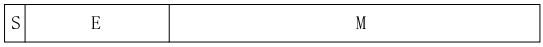
\includegraphics[width=0.9\textwidth]{IEEE754_1}
\caption{IEEE754浮点标准}
\label{fig1.1}
\end{figure}
其中S为1位符号位,E为阶码,位宽为k;M为尾数,位宽为n,且为了增加一位有效位,尾数的整数1被省略。设该格式下阶码的取值为e,尾数的取值为f,则浮点数的真是值可表示为:
\begin{equation}
x = (-1)^s * M * 2^E
\end{equation}
为了增加浮点数的可表示范围,同时为了满足标准的精度要求[12],使得阶码的真值既可表示很大的正数,也可表示与之对称的负数,阶码一般采用移码的形式表示,设偏移量为bias, bias 与阶码E的位宽k有关,一般情况下,有下式表示的关系:
\begin{equation}
bias = 2^{k-1}-1
\end{equation}
双精度浮点数在计算机中共占8个字节,全长64位,包括1位符号位S,11位偏置后的阶码E以及精度为52位的尾数M, $bias = 2^{11} - 1 = 1023$。\\
\indent 此外,该标准还规定了浮点数的舍入模式以及异常处理等,具体内容不再赘述。

\chapter{Cordic设计实现}
设计的Cordic模块输入为符合IEEE754双精度浮点数标准的角度信息,然后将其转换为定点数进行计算,最后通过转换模块将其转换为浮点数输出,同时计算$\sin$以及$\cos$。下面结合Verilog代码进行分析。由于时间有限,完成的Cordic模块仅支持$0 \sim \pi/2$范围内角度的计算。
\section{浮点数转换为定点数}
输入的双精度浮点数具有\ref{sec1.3}小节中格式,即具有1为符号位,11位偏置后的阶码以及52位尾数。为了方便进行移位操作,需要将输入的符合IEEE754浮点标准的数值转换为定点数。转换过程中,根据阶码与1023的大小来决定输入的数与1的大小,具体的转换过程具有如下形式:
{
\footnotesize
\begin{lstlisting}[language=Verilog]
if(src[61:52] < 11'd1023)
	theta[60:0] =  {1'b1,src[51:0],8'b0} >> {11'd1023-src[62:52]};
else
	theta[60:0] =  {1'b1,src[51:0],8'b0} << {11'd1023-src[62:52]};
\end{lstlisting}
}
\noindent 如上述转换代码所示,若阶码小于1023,则输入值小于1,需将尾码部分左移;阶码大于1023时相反。
\section{定点数转换为浮点数}
在将定点数转化为符合IEEE754标准的浮点数时,因为尾数部分与定点数相同,所以主要是确定转换后的阶码的值。阶码的值的确定与定点数中最大不为0的位置有关,也即计算在最左边的1之前的0的个数。为了便于编码,在计算过程中,将输入定点数以字节为单位进行统计,具体代码如下:
{
\footnotesize
\begin{lstlisting}[language=Verilog]
always @(indata[55:48])
	casex(indata[55:48])
	    8'b1xxxxxxx: zeronum_6 = 3'b000;
	    8'b01xxxxxx: zeronum_6 = 3'b001;
	    8'b001xxxxx: zeronum_6 = 3'b010;
	    8'b0001xxxx: zeronum_6 = 3'b011;
	    8'b00001xxx: zeronum_6 = 3'b100;
	    8'b000001xx: zeronum_6 = 3'b101;
	    8'b0000001x: zeronum_6 = 3'b110;
	    8'b00000001: zeronum_6 = 3'b111;
	    8'b00000000: zeronum_6 = 3'b000;
	endcase
\end{lstlisting}
}
其中\textit{zeronum\_6}表示输入数据\textit{indata}在$55 \sim 48$位范围内最高位0的个数。
最后将所有字节的统计信息求和即可求得在转换过程中需要的总的移位数。
\section{$\arctan$编码}
基于第一章节对算法的讨论,在Cordic算法求解过程中,需要的计算类型包括符号位操作、加法器、移位操作以及角度的更新等。需要的操作数包括上一次迭代的$\sin, \cos$值以及下一次需要旋转的角度数。为了便于角度更新以及实现通过移位操作即可求解新的角度的$\sin, \cos$值,我们引入一系列的$\arctan$值来简化上述迭代过程,具体来说,通过预先求解$\arctan(2^{-i})$的值来实现上述两个要求,此时仅通过简单的加减运算以及移位运算即可实现Cordic算法一次迭代的求解。
在具体实现中,预先求解的$\arctan$结果例子如下:
{
\footnotesize
\begin{lstlisting}[language=Verilog]
parameter atan_0  =
 62'b00_1100_1001_0000_1111_1101_1010_1010_0010_0010_0001_0110_1000_1100_0000_0000;
parameter atan_1  =
 62'b00_0111_0110_1011_0001_1001_1100_0001_0101_1000_0110_1110_1101_0011_1100_0000;
parameter atan_2  =
 62'b00_0011_1110_1011_0110_1110_1011_1111_0010_0101_1001_0000_0001_1011_1010_0000;
parameter atan_3  =
 62'b00_0001_1111_1101_0101_1011_1010_1001_1010_1010_1100_0010_1111_0110_1110_0000;
parameter atan_4  =
 62'b00_0000_1111_1111_1010_1010_1101_1101_1011_1001_0110_0111_1110_1111_0101_0000;
parameter atan_5  =
 62'b00_0000_0111_1111_1111_0101_0101_0110_1110_1110_1010_0101_1101_1000_1001_0100;
parameter atan_6  =
 62'b00_0000_0011_1111_1111_1110_1010_1010_1011_0111_0111_0110_1110_0101_0011_0110;
parameter atan_7  =
 62'b00_0000_0001_1111_1111_1111_1101_0101_0101_0101_1011_1011_1011_1010_1001_0111;
parameter atan_8  =
 62'b00_0000_0000_1111_1111_1111_1111_1010_1010_1010_1010_1101_1101_1101_1101_1100;
parameter atan_9  =
 62'b00_0000_0000_0111_1111_1111_1111_1111_0101_0101_0101_0101_0110_1110_1110_1111;
parameter atan_10 =
 62'b00_0000_0000_0011_1111_1111_1111_1111_1110_1010_1010_1010_1010_1011_0111_1000;
parameter atan_11 =
 62'b00_0000_0000_0001_1111_1111_1111_1111_1111_1101_0101_0101_0101_0101_0101_1100;
parameter atan_12 =
 62'b00_0000_0000_0000_1111_1111_1111_1111_1111_1111_1010_1010_1010_1010_1010_1011;
parameter atan_13 =
 62'b00_0000_0000_0000_0111_1111_1111_1111_1111_1111_1111_0101_0101_0101_0101_0101;
parameter atan_14 =
 62'b00_0000_0000_0000_0011_1111_1111_1111_1111_1111_1111_1110_1010_1010_1010_1011;
parameter atan_15 =
 62'b00_0000_0000_0000_0001_1111_1111_1111_1111_1111_1111_1111_1101_0101_0101_0101;
parameter atan_16 =
 62'b00_0000_0000_0000_0000_1111_1111_1111_1111_1111_1111_1111_1111_1010_1010_1011;
parameter atan_17 =
 62'b00_0000_0000_0000_0000_0111_1111_1111_1111_1111_1111_1111_1111_1111_0101_0101;
parameter atan_18 =
 62'b00_0000_0000_0000_0000_0011_1111_1111_1111_1111_1111_1111_1111_1111_1110_1011;
parameter atan_19 =
 62'b00_0000_0000_0000_0000_0001_1111_1111_1111_1111_1111_1111_1111_1111_1111_1101;
... ...
\end{lstlisting}
}
其中,每一个定点小数编码最高位为符号位,然后是一位整数位,剩下的60位为小数部分,$atan\_0$为$\arctan(2^0)$的计算结果,$atan\_1$为$\arctan(2^{-1})$的计算结果,剩下部分与此同理。此外,当$i$足够小时有:$\arctan(2^{-i}) \approx 2^{-i}$,因此当$i \le 20$时,用$2^{-i}$代替相应的$\arctan$值。因此,在Cordic模块中共包含了61个角度的$\arctan$值。
\section{迭代求解过程}
根据Cordic原理,其求解过程就是一系列旋转的过程,且每一次旋转都旋转不同但固定的角度。在本实验中,首先旋转$\pi/2$,接下来的每一次旋转角度都是上一次旋转角度的$1/2$,其每次旋转的角度对应上一小节中对应的$\arctan$值。然后,每一次旋转过程在Verilog中对应于一级流水线,对于双精度的Cordic算法,一次$\cos, \sin$计算需要61个时钟周期完成计算。其相邻两次迭代过程代码如下:
{
\footnotesize
\begin{lstlisting}[language=Verilog]
// cordic 55
reg [61:0] x55,y55;
reg [61:0] z55;
always @(posedge clk or negedge rst)
begin
    if(!rst) begin
         x55 <= 0;
         y55 <= 0;
         z55 <= 0;
    end
    else begin
         if(z54[61]==0)
              x55 <= x54 - {{54{y54[61]}},y54[61:54]};
         else x55 <= x54 + {{54{y54[61]}},y54[61:54]};
         if(z54[61]==0)
              y55 <= y54 + {{54{x54[61]}},x54[61:54]};
         else y55 <= y54 - {{54{x54[61]}},x54[61:54]};
         if(z54[61]==0)
              z55 <= z54 - atan_54;
         else z55 <= z54 + atan_54;
    end
end
// cordic 56
reg [61:0] x56,y56;
reg [61:0] z56;
always @(posedge clk or negedge rst)
begin
    if(!rst) begin
         x56 <= 0;
         y56 <= 0;
         z56 <= 0;
    end
    else begin
         if(z55[61]==0)
              x56 <= x55 - {{55{y55[61]}},y55[61:55]};
         else x56 <= x55 + {{55{y55[61]}},y55[61:55]};
         if(z55[61]==0)
              y56 <= y55 + {{55{x55[61]}},x55[61:55]};
         else y56 <= y55 - {{55{x55[61]}},x55[61:55]};
         if(z55[61]==0)
              z56 <= z55 - atan_55;
         else z56 <= z55 + atan_55;
    end
end
\end{lstlisting}
}
在每一级流水线中,需要完成两件事:
\begin{itemize}
\item 判断旋转到的角度与输入角度的大小,决定下次的旋转方向\\
如果输入角度大,则继续逆时针旋转,否则顺时针旋转;
\item 基于上一级流水线的结果,计算本级流水线的结果
\end{itemize}
在上述代码中,x表示待求的$\cos$, y代表带求解的$\sin$值。他们的初始化过程如下所示:
{
\footnotesize
\begin{lstlisting}[language=Verilog]
reg [61:0] x1,y1;
reg [61:0] z1;
always @(posedge clk or negedge rst)
begin
    if(!rst) begin
         x1 <= 0;
         y1 <= 0;
         z1 <= 0;
    end
    else begin
         x1 <= 62'b00_100110110111010011101101101010000100001101011110010110000000;  //0.60725293500888122
                    //10011011011101001110110110101000010000110101111001011
         y1 <= 62'b00_100110110111010011101101101010000100001101011110010110000000;
         z1 <= theta - atan_0;//
    end
end
\end{lstlisting}
}
其中x的初始值为设为0.60725293500888122。
\section{TestBench}
本次试验中,主要采用模拟验证的方式对模块进行功能验证,模拟验证即通过编写TestBench,产生输入激励,然后根据输出判断设计的功能正确性。同时还需要考虑验证覆盖率因素的影响。

\section{C++语言实现}
由于时间所限,本次仅实现了基于C++语言的32位定点数的Cordic算法。编码具有如下格式:每次旋转角度的编码由32位定点数组成,其中包括
1位的符号位,1位的整数位以及30位小数位。代码实现与上一章节的伪代码相对应。\\
输出结果为:输入为0x3243F6A9 ($\pi / 4$)时,输出为$\cos = \mathrm{0x}2D413CD(0.70710678\dots)$,$\sin = \mathrm{0x}2D413CD(0.70710678\dots)$; 输入为0x2182A470 ($\pi / 6$)时, 输出为$\cos = \mathrm{0x}367CF5D5(0.86602540\dots)$,$\sin = \mathrm{0x}20000001(0.500000000\dots)$。

这部分的代码见附录A。
\section{总结}
在本章节中,根据第一章节中对Cordic算法的讨论,简要介绍了Verilog代码的实现过程。总的来说,输入为满足IEEE754浮点标准的浮点角度值,然后将其转化为定点数进行超越函数$\cos, \sin$的求解,最后将计算结果转化为浮点数进行输出的过程。

\chapter{前端流程}
本章节主要完成Cordic模块的前端设计流程,包括基于NC的功能验证以及覆盖率检查,基于DC的逻辑综合,生成.sv网表文件。
\section{工具简介}
本小节将对前端设计流程中用到的工具软件进行简要说明,包括NC,DC等。
\subsection{NC}
NC-Verilog是Candence公司的Verilog数字逻辑模拟器,具有运行快、精度高、调试功能强大、使用灵活等优点,是业界公认的黄金模拟器。NC-Verilog的运行分为两个步骤,首先是编译,检查语法错误等,然后模拟执行。NC-Verilog使用NCC技术,提高了模拟的性能减少了内存的使用。采用INCA架构,具备了支持多种HDL语言、多设计层次、数模混合设计的能力。

运行流程包括:建立列表文件,列表文件包含激励信号;建立配置文件,以一个脚本的形式对NC进行配置,包括启动GUI界面、开启覆盖率统计、访问权限等设置;运行NC-Verilog,以上一步的配置启动NC;波形查看与调试,可以通过“shm\_open”和“shm\_probe”两个命令来保存波形,并且可以查看信号的波形以及逻辑结构图等,这一步主要通过查看波形以确定模块的正确性;查看覆盖率,这一步同样需要一个TCL脚本文件进行配置,并借助ICCR软件进行分析;导出VCD文件,可以通过tcl脚本或NC软件或“dumpfile”“dumpvars”来完成。以上就是功能验证部分的工作流程。 
\subsection{DC}
DC工具是Synopsys公司的逻辑综合工具,完成Verilog文件到RTL级网表的转换,并可根据不同的约束条件进行不同的综合。PT软件是Synopsys公司提供的静态分析工具,可以完成网表的静态时序分析,可以报告最长和最短路径等。

逻辑综合流程包括:建立综合环境,该环境包括列表文件、时序约束文件、运行配置文件以及启动设置文件等,运行配置文件包括了模块顶层模块的设置等,启动文件包括了综合过程中用到的库以及库的路径等信息;对模块进行综合;更改设计约束,得到不同的综合结果;对综合结果进行静态时序分析。
\section{功能验证}
\subsection{基于NC的功能验证}
首先建立列表文件,Cordic模块共包含3个文件:{\itshape LZB.v, Sin\_Cos\_Func.v, Sin\_Cos\_Func\_tb.v},其中\textit{LZB.v}为定点数转浮点数用到的模块,\textit{Sin\_Cos\_Func.v}为Coridc的实现文件,包括输入浮点数转定点数、$\sin, \cos$求解以及输出控制等功能的实现,最后一个文件\textit{Sin\_Cos\_Func\_tb.v}为模块的TestBench文件,其包括时钟信号的产生以及输入激励的设定等部分。列表文件内容如下:
\begin{lstlisting}[language=Verilog]
`include ``../Sin_Cos_Func_tb.v"
`include ``../Sin_Cos_Func.v"
`include ``../LZD.v"
\end{lstlisting}
其中以相对路径对文件进行搜索。\\
\indent 然后建立NC的配置文件如下:
{
\footnotesize
\begin{lstlisting}[language=tcl]
filelist.v -s +gui +access+r
//ignore sdf annotations
+nospecify
//invoke 64bit verion
//+nc64bit
+ncnowarn+CUNGL1
+ncnowarn+NONPRT
+frofile
+nccoverage+all
+nccoveragewrite
\end{lstlisting}
}
\noindent 其中最后面两个命令为控制生成覆盖率信息。最后利用如下脚本命令运行NC:\\
\begin{verbatim}
#! /bin/bash
ncverilog -f ncverilog.options &
\end{verbatim}
\subsection{功能验证波形}
图\ref{figure3.1}是NC工具得到的Cordic模块的仿真波形。
\begin{figure}[!hbtp]
\centering
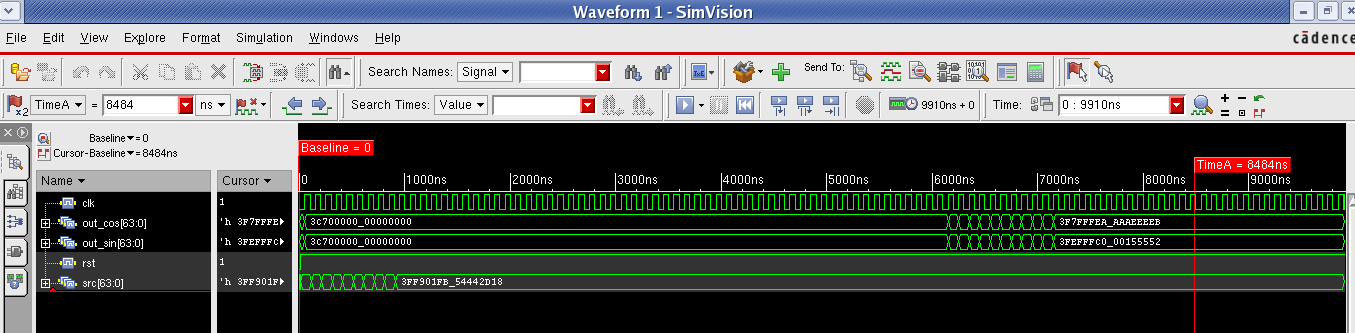
\includegraphics[width=0.9\textwidth]{NC1}
\caption{NC输出波形图}
\label{figure3.1}
\end{figure}\\
图中显示了输入为64'h0000\_0000\_0000\_0000, 64'h3F21\_DF46\_A252\_9D00, 64'h\\3F80\_0000\_0000\_0000, 64'h3F91\_DF46\_A252\_9D38,64'h3FE9\_21FB\_5444\_2D18等角度时的输出。为了验证模块的正确性,图显示了对应的输出。
\begin{figure}[!hbtp]
\centering
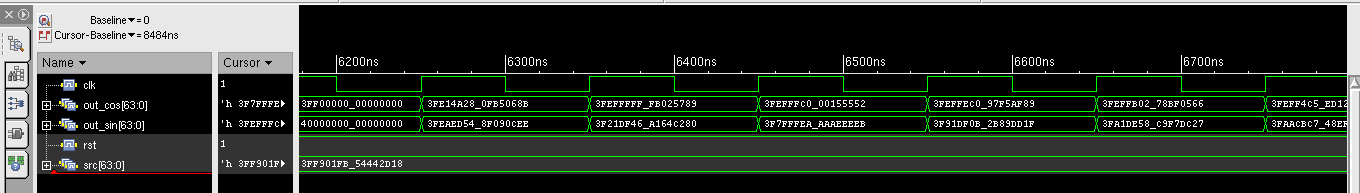
\includegraphics[width=0.9\textwidth]{NC2}
\caption{模块的计算结果}
\label{figure3.2}
\end{figure}
从图\ref{figure3.2}中可以看出,当输入为0时,输出的cos值为0x3FF0\_0000\_0000\_0000,然而输出的sin值为0x4000\_0000\_0000\_0000,具有较大的误差;输入为64'h3FE9\_21FB\_5444\_2D18 (0.78539...),即输入为$\pi/4$时,cos输出为:0x3FE6\_A09E\_667F\_3BCC, sin输出为:0x3FE6\_A09E\_667F\_3BCC。通过波形,我们可以看出,设计的Cordic在边界条件以外的时候具有较高的计算精度,由于时间有限,对于边界情况下计算误差较大的情况还有待进一步改进。

表\ref{table1}给出了具体的输入数值以及运算结果的对应情况:
\begin{table}[!hbtp]
\centering
\caption{功能验证结果}
\label{table1}
\begin{tabular}{ccc}
\toprule
\multirow{2}{*}{输入} & \multicolumn{2}{c}{输出} \\
\cline{2-3}
 &  Cos   & Sin \\
\midrule
64'h00000000\_00000000  & 0x3FF00000\_00000000  & 0x40000000\_00000000 \\
64'h3F21DF46\_A2529D00  & 0x3FE14A28\_0FB5068B  & 0x3FEAED54\_8F090CEE \\
64'h3F800000\_00000000  & 0x3FEFFFFF\_FB025789  & 0x3F21DF46\_A164C280 \\
64'h3F91DF46\_A2529D38  & 0x3FEFFFC0\_00155552  & 0x3F7FFFEA\_AAAEEEEB \\
64'h3FA1DF46\_A2529D39  & 0x3FEFFEC0\_97F5AF89  & 0x3F91DF0B\_2B89DD1F \\ 
64'h3FAACEE9\_F37BEBD6  & 0x3FEFFB01\_78BF0566  & 0x3FA1DE58\_C9F7DC27 \\ 
64'h3FE0C152\_382D7366  & 0x3FEBB67A\_E8584CAA  & 0x3FE00000\_00000000 \\
64'h3FE921FB\_54442D18  & 0x3FE6A09E\_667F3BCC  & 0x3FE6A09E\_667F3BCC \\
64'h3FF0C152\_382D7366  & 0x3FDFFFFF\_FFFFFFFD  & 0x3FEBB67A\_E8584CAB \\
64'h3FF901FB\_54442D18  & 0x3F7FFFEA\_AAAEEEEE  & 0x3FEFFFC0\_00155552 \\
\bottomrule

\end{tabular}
\end{table}

\subsection{覆盖率结果及分析}
为了保证功能验证部分对模块的覆盖情况,我们借助ICCR工具对覆盖率进行统计。图\ref{figure3.3a}是模块的覆盖率结果,图\ref{figure3.3b}是各block以及翻转覆盖率结果,图\ref{figure3.3c}显示了具体的未覆盖的语句。

从图\ref{figure3.3a}中可以看出,模块覆盖率达到95\%, 从图\ref{figure3.3b}可以看出LZD功能单元的block覆盖率较低,借助工具的统计信息,图\ref{figure3.3c}显示了导致该覆盖率较低的原因,从图中可以看出,源文件中的casex语句中存在大量不确定性数值选项,如8'b001xxxxx,也正因为这些语句的存在导致了覆盖率较低。一种提高覆盖率办法是列出所有的准确选项,但这样会导致程序可读性变差,因此这里不对这个地方进行修改。
\begin{figure}[!hbtp]
\centering
\subfigure[Module覆盖率]{
\label{figure3.3a}
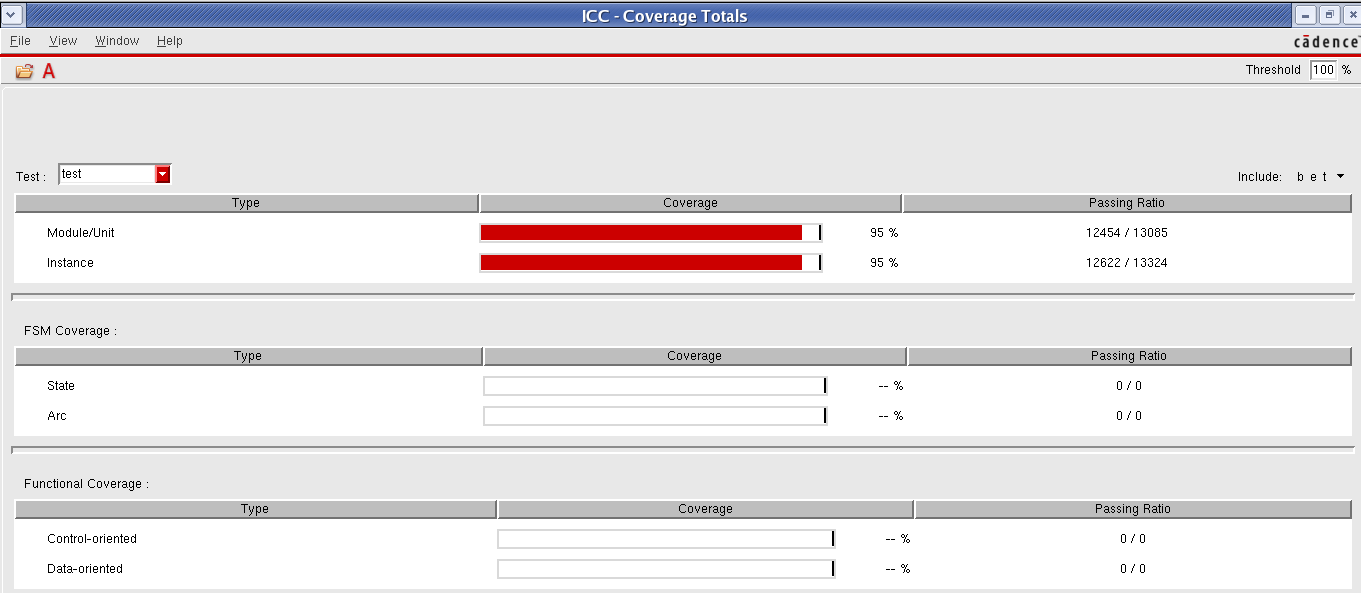
\includegraphics[width=1.0\textwidth]{iccr1}
}\\
\subfigure[Block及翻转覆盖率等]{
\label{figure3.3b}
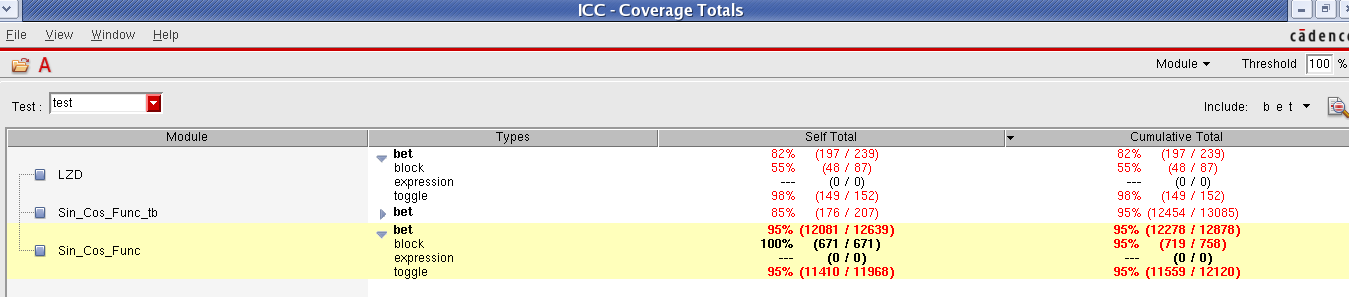
\includegraphics[width=1.0\textwidth]{iccr2}
}\\
\subfigure[未覆盖语句分析]{
\label{figure3.3c}
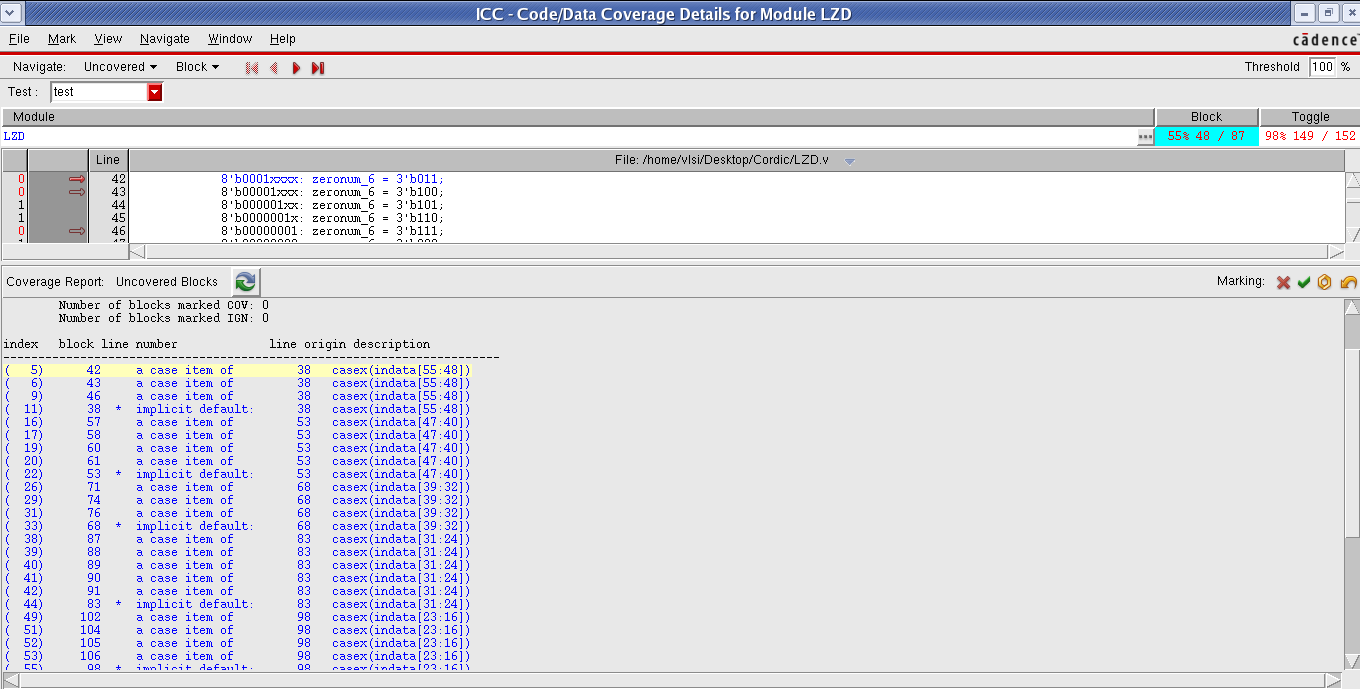
\includegraphics[width=1.0\textwidth]{iccr3}
}
\caption{覆盖率统计结果}
\label{figure3.3}
\end{figure}
\section{逻辑综合}
本小节将给出Cordic模块的综合结果,包括时序、面积、功耗等性能参数,且生成.sv格式的网表文件用于后端物理设计。
\subsection{基于DC的逻辑综合}
首先通过自定义的new\_dc命令建立综合环境,并拷贝进filelist.tcl、synopsys.sdc、top.tcl、.synopsys\_dc.setup等文件,这些文件中包含了运行DC所需的模块代码、时序约束、DC运行配置、库文件以及搜索路径等信息。\\
\indent filelist.tcl包含了Verilog代码,其内容如下:
{
\footnotesize
\begin{lstlisting}[language=tcl]
analyze -f VERILOG -library DEFAULT ../Sin_Cos_Func.v
analyze -f VERILOG -library DEFAULT ../LZD.v
\end{lstlisting}
}
synopsys.sdc包含了综合时所需的时序约束等信息,包括时钟周期、don't touch网络、输入输出延时、最大延时等。具体内容如下:
{
\footnotesize
\begin{lstlisting}[language=tcl]
set clk_period 1.5

# clock definition

create_clock -name {clk} -period $clk_period -waveform {0  0.55} [get_ports {clk}]     

# set dont touch

set_dont_touch_network [get_clocks {clk}]

#####################################################

set_clock_transition   0.05 [get_clocks { clk }]

set_clock_uncertainty  0.1 -hold [get_clocks { clk }]

set_clock_latency 0.1 [get_clocks {clk}]

#set_driving_cell -lib_cell BUFX2TL -library 
#scx2_smic_013g_lvt_tt_1p2v_25c [remove_from_collection [all_inputs] clk reset]

set_load 0.1 [all_inputs]

set_input_delay 0 -clock clk [all_inputs]

set_output_delay 0 -clock clk [all_outputs]

# Constrain combinational logic.

set_max_delay 1.2 -from [all_inputs] -to [all_outputs]
\end{lstlisting}
}
.synopsys.setup是一个隐藏文件,内容包括了综合库、目标库、链接库、符号库以及搜索路径等信息。Top.tcl是一个脚本文件,控制了DC的启动方式以及综合配置等,包括操作环境、源文件的导入以及综合结果的输出等。其内容略。

\subsection{逻辑综合结果及其优化}
在对设计的Cordic模块进行综合时,首先设置时钟周期为1.5ns,的到图\ref{figure3.4}所示的时序报告。从图中可以看出,当时钟周期设为1.5ns时,设计违反时序,表现为slack为负值。在接下来的综合过程中,考虑到需要为后端物理设计预留充分的时序裕度,我们将时钟周期设为3ns进行综合。图\ref{figure3.5}所示为增加时钟周期后的时序综合结果。同时,图\ref{figure3.6}所示为时钟周期为3ns时的面积、功耗综合结果。

为了体现时序-面积之间的制约关系,表\ref{table2}表示时钟周期为1.5ns, 2ns, 2.5ns, 3ns时的面积功耗结果。
\begin{figure}[!hbtp]
\centering
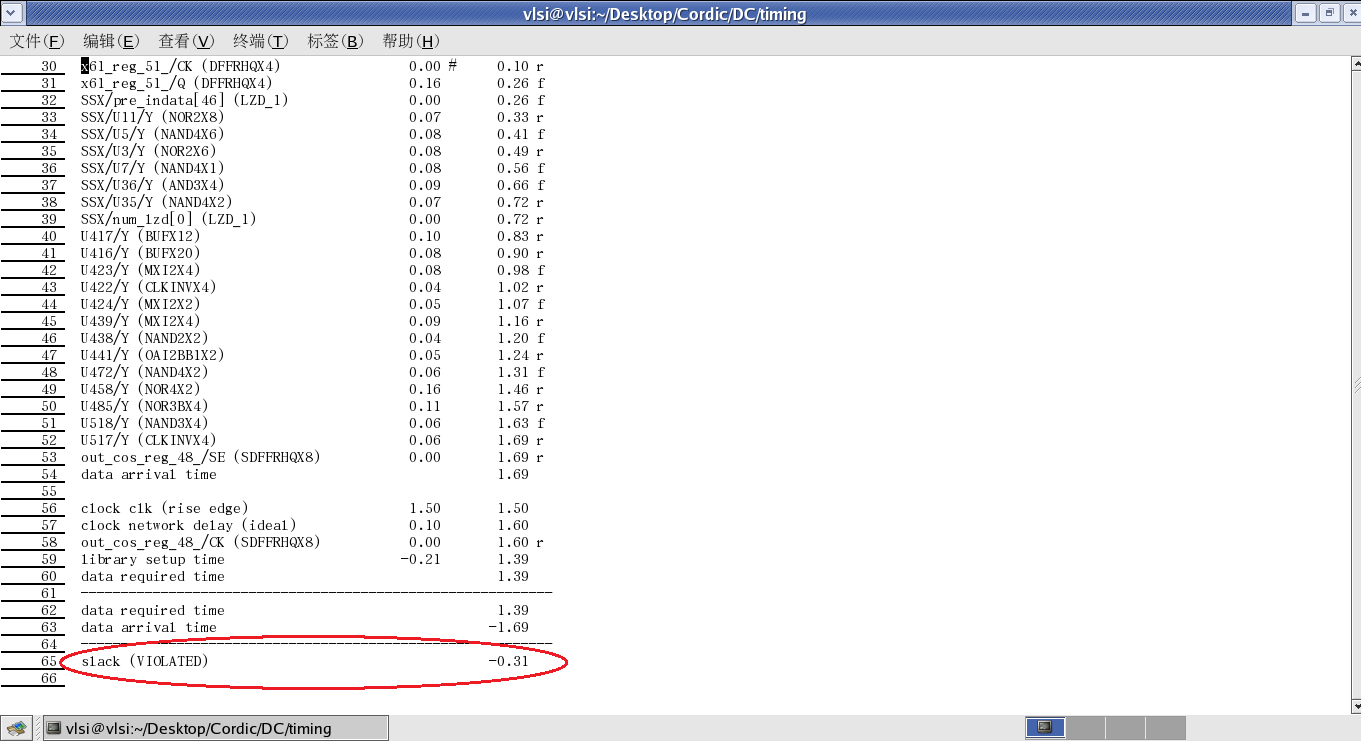
\includegraphics[width=1.0\textwidth]{time1}
\caption{时钟周期为1.5ns时的时序报告}
\label{figure3.4}
\end{figure}
\begin{figure}[!hbtp]
\centering
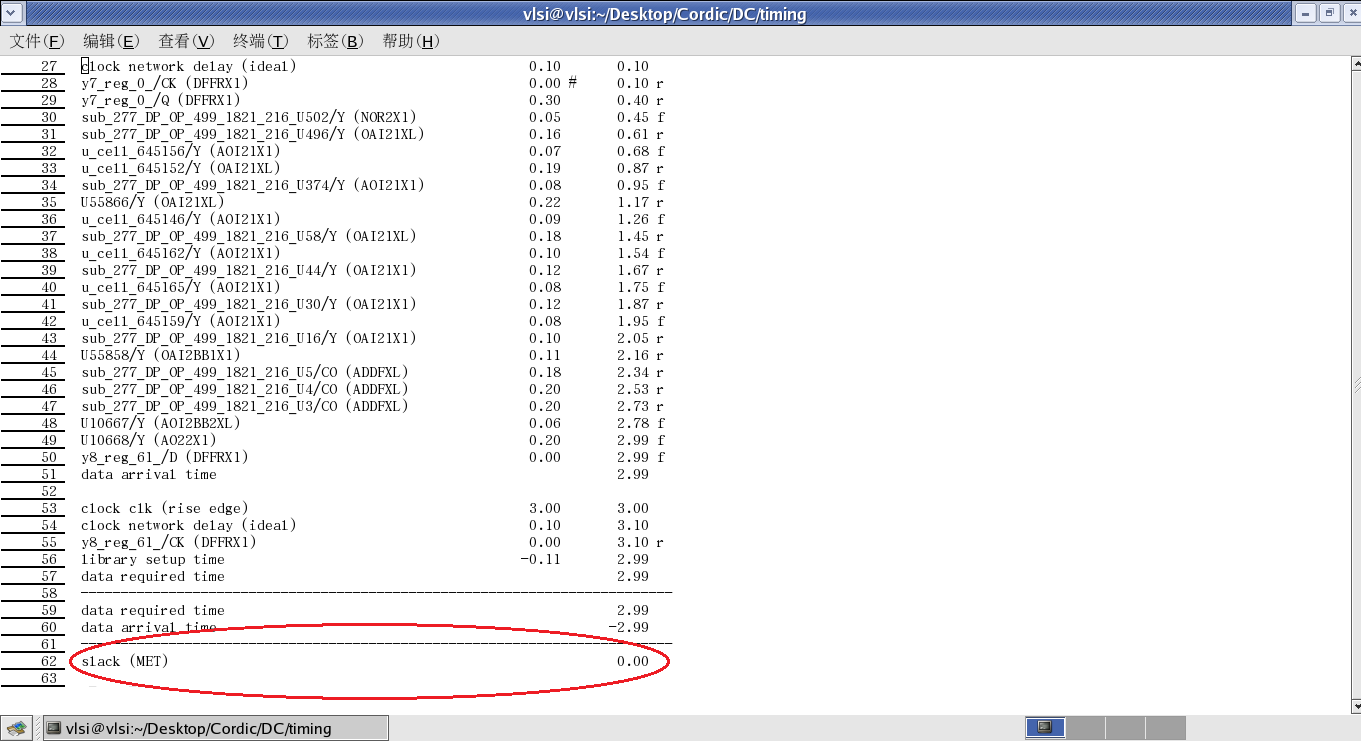
\includegraphics[width=1.0\textwidth]{time2}
\caption{时钟周期为3ns时的时序报告}
\label{figure3.5}
\end{figure}
\begin{figure}[!hbtp]
\centering
\subfigure[时钟周期为3ns时的面积结果]{
\label{figura3.6a}
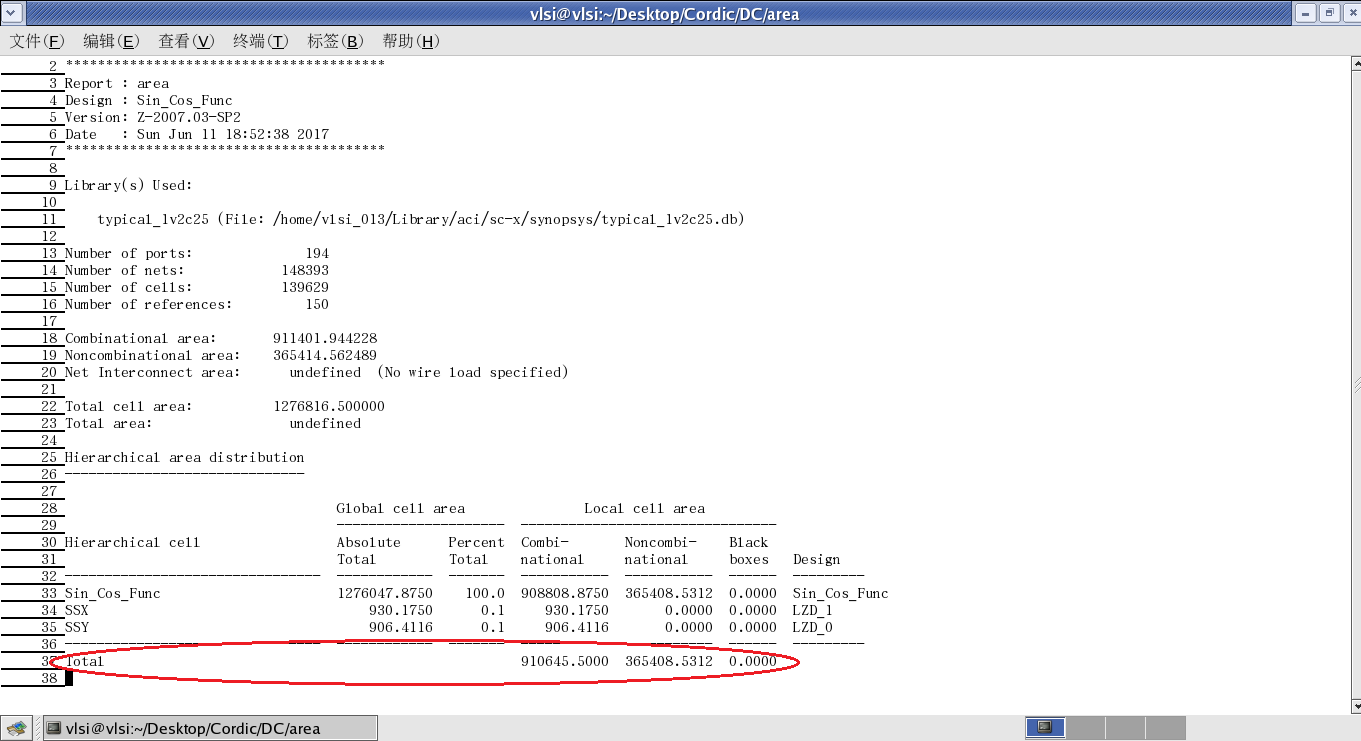
\includegraphics[width=1.0\textwidth]{area}
}
\\
\subfigure[时钟周期为3ns时的时序结果]{
\label{figure3.6b}
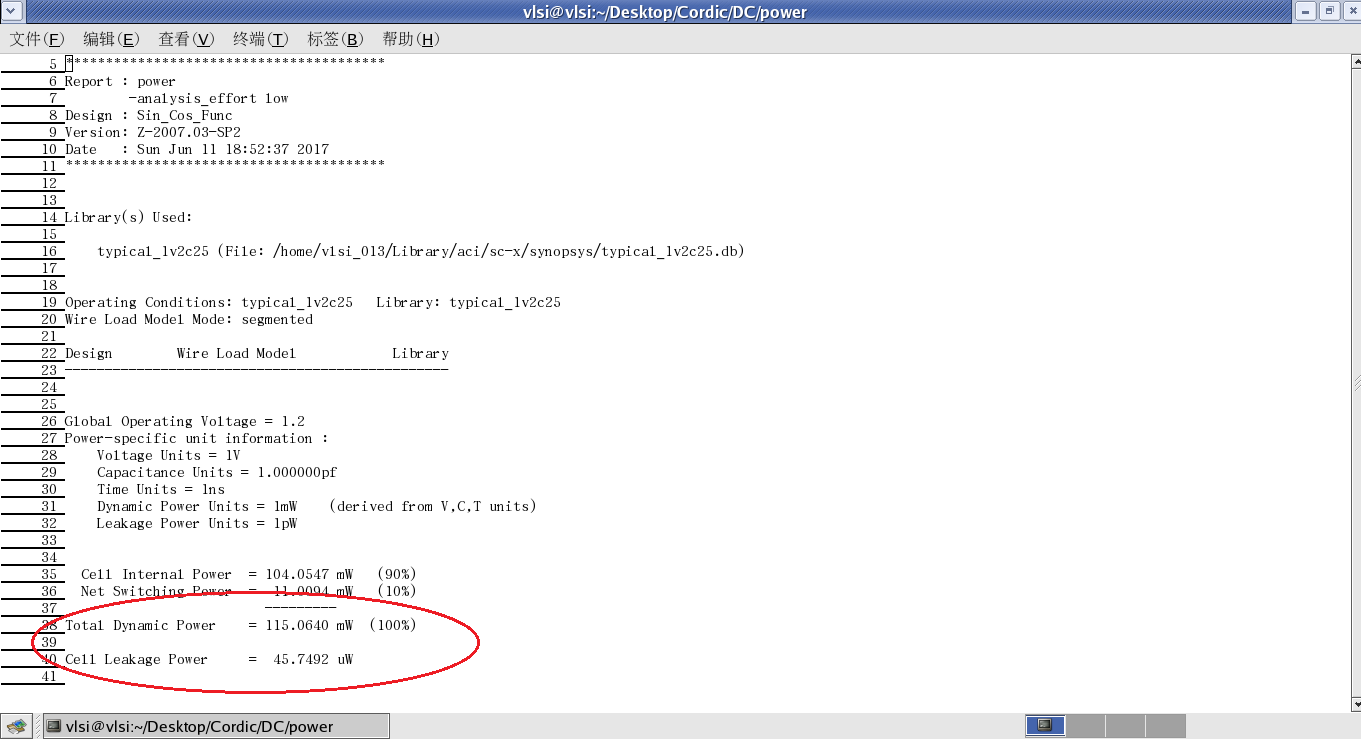
\includegraphics[width=1.0\textwidth]{power}
}
\caption{时钟周期为3ns时的综合结果}
\label{figure3.6}
\end{figure}
\begin{table}[!hbtp]
\centering
\label{table2}
\caption{不同时钟周期下的综合结果}
\begin{tabular}{ccc}
\toprule
时钟周期  &  面积($um^2$)      &    功耗(仅动态功耗)   \\ 
\midrule
1.5ns    &  1575840.6 & 300.8mW  \\
2ns      &  1329760.1 & 179.8mW  \\
2.5ns    &  1298497.4 & 139.2mW  \\
3ns      &  1276816.5 & 115.1mW  \\
\bottomrule
\end{tabular}
\end{table}
\section{静态时序分析}
在本小节,静态时序分析主要基于Prime Time工具软件实现。
\subsection{基于PT的静态时序分析}
基于PT的静态时序分析主要操作流程如下:
\begin{itemize}
\item 新建目录PT,然后将逻辑综合后的.sv网表以及.spef文件拷贝至该目录;
\item 编写脚本primetime.scrip,其中设定了PT参考的时序文件、顶层模块名以及报告的输出的等;
\item 执行命令\verb|pt_shell -file primetime.script| | \verb|tee primetime.log|;
\item 分析PrimeTime给出的时序报告
\end{itemize}
\subsection{PT结果}
图\ref{figure3.7}显示了PT的时序报告的内容,在文本中搜索是否有VIOLATE的情况,结果表明,综合后的网表满足时序约束。
\begin{figure}[!hbtp]
\centering
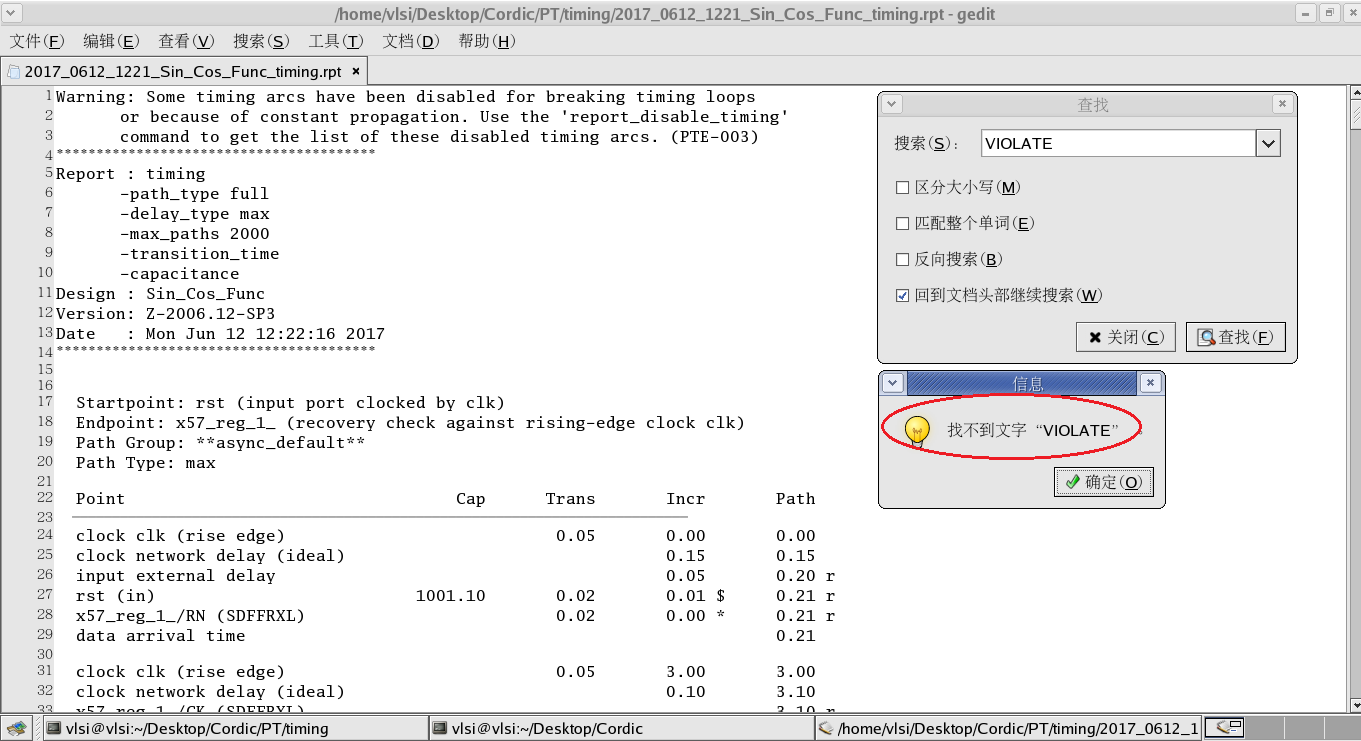
\includegraphics[width=1.0\textwidth]{PT1}
\caption{PT静态时序分析结果}
\label{figure3.7}
\end{figure}

\section{总结}
本章节主要内容是对Cordic模块的前端设计流程以及各阶段的结果,包括基于NC的功能验证、基于DC的逻辑综合等。表\ref{table1}包含了功能验证的结果,包括边界条件验证以及其它特殊点的验证等,结果表明,在范围$0 \sim \pi/2$范围内,计算结果良好,误差较小,但对于边界情况下,sin值的计算误差较大,这是需要进一步改进的地方。对于逻辑综合,首先设置了时钟周期为1.5ns的情况下的综合,时序报告表明,此时违反时序约束,因此在后续的综合过程中,将时钟周期增加,又考虑到后端物理设计同样需要充足的时序裕度,因此,在本次实验中,时钟周期最终被设定为3ns,综合结果在图\ref{figure3.5}以及\ref{figure3.6}中给出。同时,表\ref{table2}给出了在不同时钟周期约束下的综合结果,包括面积、功耗等。从该表中可以看出,时钟周期越大,则面积资源开销就越小,同时动态功耗也越小,这是符合实际情况的。接下来,将利用综合得到的.sv网表进行物理设计,相关内容在下一章节展开。

\chapter{后端流程}
本章节主要完成Cordic模块的后端设计流程,包括基于Encounter的布局布线等、基于Calibre的DRC/LVS检查等。
\section{后端设计流程简介}
本小节将简要介绍数字集成电路的后端设计的各个流程,主要包括以下四个部分。

布局规划(FloorPlan)。布局规划就是放置芯片的宏单元模块,在总体上确定各种功能电路的摆放位置,如IP模块、RAM、I/O引脚等。布局规划能影响芯片最终的面积,并可设定模块对于芯片面积的使用率以及标准单元的排列方式等。具体的,还包括,I/O pin的摆放、电源环的摆放以及电源所处的金属层、标准单元的生成等。

时钟树综合(CTS)。由于时钟信号在数字芯片中起到全局指挥作用,因此它的分布应该是对称式的连接到各个寄存器单元,从而使得时钟从同一个时钟源到达各个寄存器时,时钟延时差异(Skew)最小。为实现Skew最小,会对时钟路径进行插入Buffer。

布线(Routing)。在完成时钟树综合后,就可以对普通信号进行布线。在此过程中,需要注意避免线间耦合效应的产生,且密度不能过大,可通过填充金属等来实现。

版图物理设计。对完成布线的物理版图进行功能和时序上的验证,验证过程包括很多项目,如LVS(Layout Vs Schematic)验证,即将版图与逻辑综合后的门级电路图进行对比验证;DRC(Design Rule Checking),设计规则检查,检查连线间距、连线宽度等是否满足工艺要求;ERC(Electrical Rule Checking),电器规则检查,检查短路和开路等电器规则违反情况。物理图版验证完成后,即可将物理班图以GDS文件格式的形式交由芯片代工厂进行实际生产,然后再进行封装和测试。

从布局规划到布线的所有流程主要基于Encounter工具软件完成,后面的版图物理设计主要基于Calibre工具软件完成。
\section{实验原理}
本实验主要基于EDA工具完成击沉电路的物理设计流程,物理设计流程的主要内容是布局布线。该流程大致可分为三个阶段,一个是准备阶段,主要包括逻辑网表、时序约束、工艺文件、单元库等设计数据的准备;二是设计与优化阶段名主要包括布局规划、布局、布局优化、时钟树综合、布线、布线优化等;三是验证和签核阶段,主要包括寄生参数提取、静态时序分析、物理规则检查等。
\subsection{数据准备}
需要准备的数据可分为库文件以及设计数据两类。库文件定义了具体工艺下最好与最差以及典型情况下的时序参数,此外还有提供LEF视图的库文件等。设计数据包括综合后的逻辑网表、包含时序约束的SDC文件以及定义I/O Pad位置的TDF文件等。综合后的逻辑网表包含芯片的门级逻辑描述,但不包括位置、大小、延时等物理信息,是物理设计的起点。SDC文件定义了设计的时序约束,包括时钟定义、输入输出延时、路径约束以及驱动能力等,是进行时序优化的依据。TDF文件通常用于I/O管脚及其排列位置等信息。

此外,物理设计流程所包含的各个步骤之间通过save design的方式来实现数据交互。
\subsection{设计与优化}
\noindent \textbf{布局规划}

布局规划是布局布线设计流程中非常重要的一环,有展平式和层次式两种方式。展平式布局规划具有操作简单、布局布线快和面积利用率高等优点。而层次式布局规划具有时序收敛快、互连延时小等优点,但操作较为复杂,面积利用率不高。本次实验仅以展开式布局规划的方式进行展开。

展平式布局规划,主要是确定芯片的尺寸、标准单元的排列方式、硬核和全定制单元的位置、电源/地/时钟/关键数据总线的分布以及布局布线区域的约束等。总之,布局规划的目的就是保证布线拥塞少、性能达标的前提下,最大限度的减少芯片面积、降低设计复杂度。

(1)芯片尺寸的确定

芯片尺寸的大小决定了投片成本的大小。芯片的面积主要包括I/O面积和内核面积。I/O面积是指I/O Buffer单元和I/O Pad所占的面积,内核面积是指除I/O外其它逻辑功能单元所占的面积,在I/O和内核之间通常还有最小间距设计约束。

I/O部分的面积主要受I/O单元个数、Pad的最小间距以及I/O单元与内核逻辑单元最小间距的约束。一般有两种摆放方式,一种是平行方式,这种方式适合Pin脚数目较少的情况;另一种方式是交错排列方式以减少芯片面积,这在Pin脚数目较多时比较常用。

芯片面积的设置主要是内核面积的设置,可以采用“先紧后松”的方式,将初始的内核面积设小一点,内核利用率设高一点,然后再根据布局布线的拥塞程度逐渐放大。硬核数目少、面积小的设计,初始利用率可设为70%~80%,硬核数目多,面积大的设计,初始利用率可设为50%~60%。

(2)标准单元的排列

标准单元为等高不等宽的预定制单元,可以按行水平放置,也可以按列垂直放置,这主要根据工艺中Metal1的优先方向来确定。不管水平方式还是垂直方式,标准单元的排列又有非背靠背和背靠背两种方式。非背靠背方式下各行之间有额外的布线通道,各行有各行的电源地线,但单元可利用的面积少一些;背靠背方式下各行之间没有布线通道相邻两行共用电源或地线,单元可利用面积可达100%。在布线金属层较多的情况下,背靠背的方式用的较多,有利用减少芯片面积。

(3)硬核的放置

在硬核数目较多、面积较大的设计中,硬核的放置尤为重要,对布局布线结果影响非常大。硬核的放置经验有:安硬核的特殊要求放置,比如数字电路与模拟电路分开放置;按流水线或数据流的先后顺序来放置;按所属模块放置,属于同一模块的硬核应就近放置;尽量靠边角放置,引脚尽可能朝里,这样有利于五局布线优化,并减少不必要的缓冲器单元或跨硬核的长线。

(4)电源和地的分布

随着工艺减少,内核电路的工作电压越来越低,电路的额噪声容限减少,而且金属线宽减少,线长增加,电源地上的欧姆电压降对电路性能的影响变得越来越严重。因此需要为芯片中每个电路单元提供稳定电压和充足电流。电源地分布网络的设计需要达到以下三个目标:

尽量降低IR Drop引起的电压瞬间,减少对电路延时的影响;

均匀分配电流密度,避免发生芯片局部过热现象以及电子迁移效应;

提供足够的ESD保护能力。

围绕上面三个主要目标,电源地分布网络的设计需要完成以下几个工作:

a. 确定各类电源地I/O Pad的数据及位置;

b. 确定I/O部分电源地的供给方式以及各类电源的隔离方式;

c. 设计内核模块中模拟电源地的分布网络,并确定电源地网络所用的金属层与线宽;

d. 涉及内核模块中数字电源地的分部网络,并确定金属层与线宽。

等。

(5)布局布线区域的约束设置

放置好硬核并且规划后电源地网络后,还需要对布局布线的区域设置约束。对布局区域的约束有Hard Blockage和Soft Blockage两种:前者区域内不允许放置任何标准单元,而后者区域内仅不允许放置除缓冲器/反相器外的任何标准单元。

\noindent \textbf{布局}

布局规划完成后,就可以开始布局了。布局是根据SDC时序约束条件,将标准单元及硬核模块按照要求排列在标准单元行或一定区域内,并去除重叠现象。

设置布局选项主要是选择布局的优化模式:拥塞驱动、时序驱动、功耗驱动、压降驱动,或者兼而有之。一般选择前两类驱动方式,除非对于功耗、压降等要求非常严格。

预布局优化的工作主要是进行快速布局以得到连线信息,从而优化逻辑网表,为优化布局打下基础。布局阶段的主要工作是使用gate sizing, cell moving, buffer/inverter insertion, net splitting以及gate duplication等技术进行时序和拥塞优化。


\noindent \textbf{布局优化和时钟树设计}

本阶段工作主要是在布局结果的基础上对时序和时钟作进一步优化,并且对长线和串扰进行预防。

时钟树综合时,最好设置为同时考虑最坏和最好条件下的时钟偏差,使两种条件下的时钟偏差较为接近,以避免出现一种条件下优化的时钟偏差在另一种条件下急剧恶化的情况。时钟网的翻转率最高,对耦合电容敏感,因此减少时钟线网的耦合噪声,需要将其布线宽度加大,间距拉开。

布局结束后,可以导出设计的线负载模型,反馈给前端综合工具使用,从而使综合结果更符合实际。


\noindent \textbf{布线}

自动布线是完成全局布线、线轨分配和详细布线。优化布线可以较少连线长度、减少转层次数。所有线网都完成布线后,需要对时钟树再进行优化,以改善时钟偏差。	
	
\section{PD流程及结果}
PD流程主要包括FloorPlan, 布局与CTS布线,布线, 物理验证几个步骤,下面对这几个步骤进行详细说明。 
\subsection{布局规划}
\noindent{\bfseries 基于Encounter的Floorplan的主要操作流程包括}:
\begin{itemize}
\item 读入设计,即综合网表\\
	同时设置时序库、LEF视图库、时序约束等;
\item 布局规划\\
	在这一步设置Core的使用率为0.6,边界为20um,并设置标准单元的排放方式为背靠背;
\item 添加引脚信息\\
	设置引脚的位置,输入信号在左,输出信号在右,以及间距为0.2um;
\item 添加电源环\\
	添加电源环,并设置电源环距离边界的距离为4um以及线宽为5um、线间距为2um等参数;
\item 为标准单元扩展出电源地
\item 保存Floorplan的设计结果
\end{itemize}
\noindent {\bfseries FloorPlan实验结果}:\\
\indent 图\ref{figure4.1a}为Floorplan的结果, 图\ref{figure4.1b}为细节图,从途中可以看出,floorplan后设计中包含了标准单元、电源环等。
\begin{figure}[!hbtp]
\centering
\subfigure[Floorplan结果]{
\label{figure4.1a}
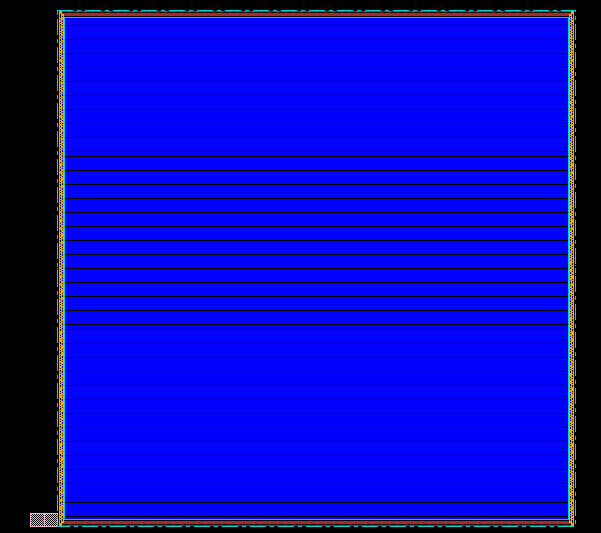
\includegraphics[width=0.95\textwidth]{floorplan7}
}
\\
\subfigure[Floorplan结果细节图,包括了电源环、标准单元等]{
\label{figure4.1b}
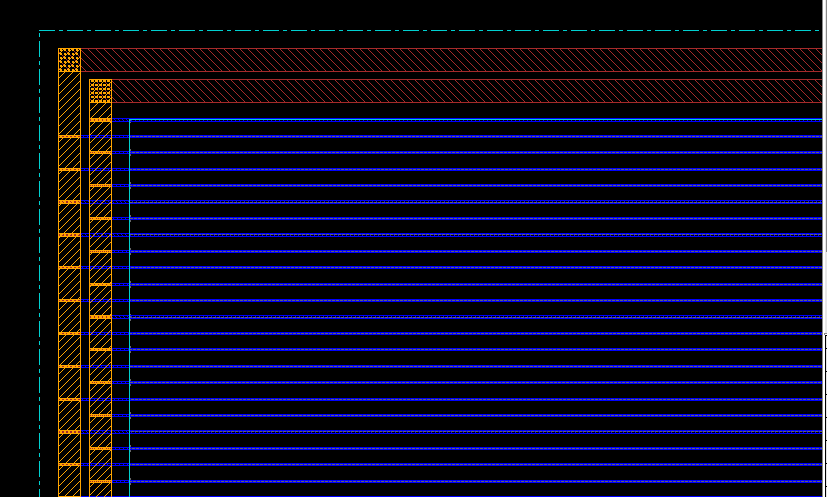
\includegraphics[width=0.95\textwidth]{floorplan8}
}
\caption{Cordic模块的布局规划结果}
\label{figure4.1}
\end{figure}
\subsection{布局以及CTS布线}
\noindent{\bfseries 基于Encounter的布局以及CTS布线的主要操作流程包括}:
\begin{itemize}
\item 读入Floorplan的设计结果\\
	Design -> Restore Design -> OK
\item 在布局之前,设置操作模式\\
	在encounter命令行下,利用setPlaceMode设置以下选项:
\begin{description}
\item[-congMediumEffort] 设置解决拥塞的努力程度为中等;
\item[-timingdriven] 设置为时序驱动的布局;
\item[-doCongOpt] 设置为开启拥塞优化;
\item[-maxDensity] 设置最大密度,这里设置为80\%;
\item[-noAssignIoPins] 设置引脚的排列,这里关闭软件对引脚的排放;
\item[-clkGateAware] 考虑时钟门控; 
\end{description}
\item 初步布局
\item 布局完成后进行CTS前的时序分析
\item 进行布局优化\\
布局优化过程如下:
\begin{itemize}
\item 设置优化选项\\
	setOptMode -fixDRC -mediumEffort -fixFanoutLoad -maxDensity 0.8
\item 利用\verb|optDesign -preCTS|进行优化
\end{itemize}
\item 保存database
\item 进行时钟树综合\\
时钟树综合的过程,又包含以下几个步骤:
\begin{itemize}
\item 设置CTS模式,指定某些选项,包括金属层、间距等
\item 创建时钟树spec文件
\item 制定spec文件
\item 时钟树综合,并插入buffer, 查看延时信息等,并根据输出的ctsrpt文件对综合结果进行分析
\end{itemize}
\item 进行CTS综合后的时序分析\\
首先将理想延时转化为传播延时,然后进行更加准确的延时分析\\ 
\verb|set_propagated_clock [all_clocks]|
\item 对设计进行CTS综合后的优化\\
\verb|optDesign -postCTS|
\item 保存database
\end{itemize}
\noindent {\bfseries 布局以及CTS综合结果}:\\
\indent 图\ref{figure4.2}到图\ref{figure4.4}表示了对Cordic模块的布局以及CTS综合过程的结果。其中图\ref{figure4.3}表示在布局过程中,对布局优化前后的时序分析结果,从截图中可以查看出,优化后的时序明显变好,但其代价就是模块的密度增加,由59\%升高到74.717\%。
最后,图\ref{figure4.4}展示了时钟树综合后的时钟网络结构,从其中可以明显看出,CTS综合后在时钟网络中增加了不同层级的Buffer。此外,该图中还包含了输入延时信息,即图中红圆圈处。

\begin{figure}[!hbtp]
\centering
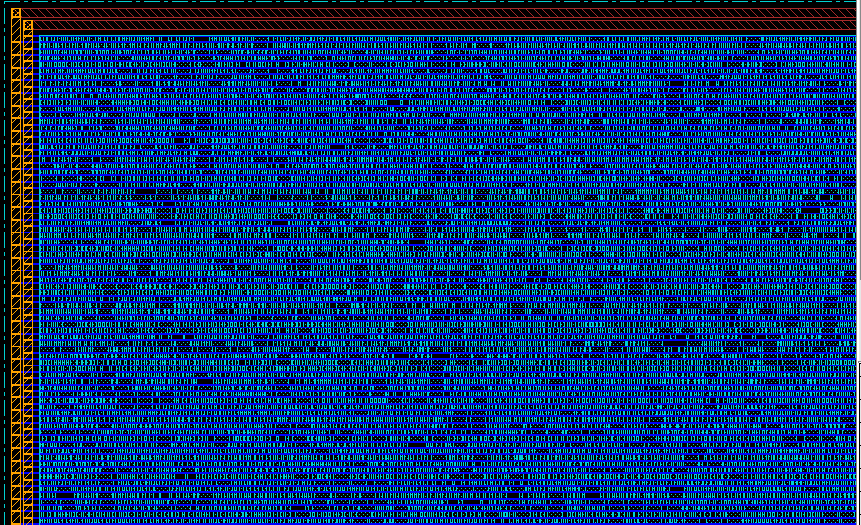
\includegraphics[width=0.85\textwidth]{CTS1}
\caption{Route之后,CTS之前的结果}
\label{figure4.2}
\end{figure}

\begin{figure}[!hbtp]
\centering
\subfigure[布局优化前的时序分析]{
\label{figure4.3a}
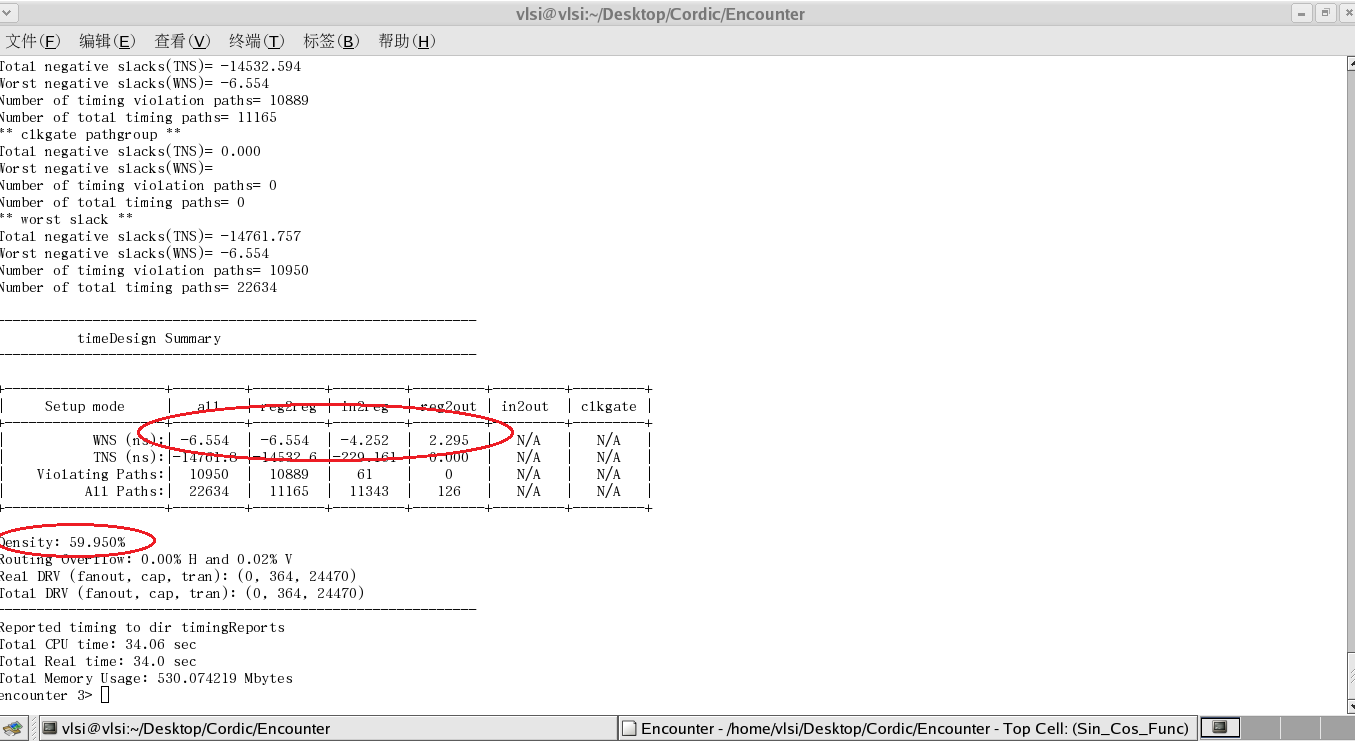
\includegraphics[width=0.9\textwidth]{CTS3}
}
\\
\subfigure[布局优化后的时序分析]{
\label{figure4.3b}
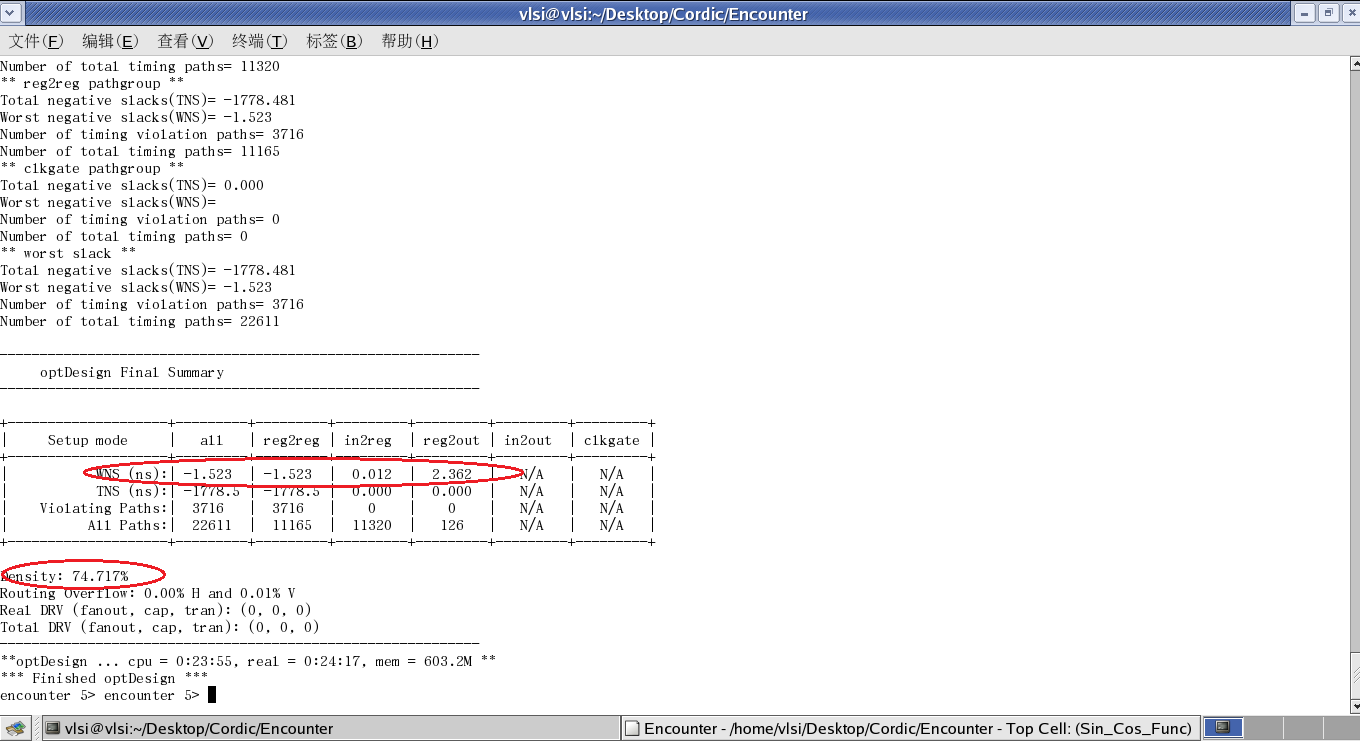
\includegraphics[width=0.9\textwidth]{CTS4}
}
\caption{布局过程中的时序结果对比}
\label{figure4.3}
\end{figure}

\begin{figure}[!hbtp]
\centering
\subfigure[CTS综合后的时钟树]{
\label{figure4.4a}
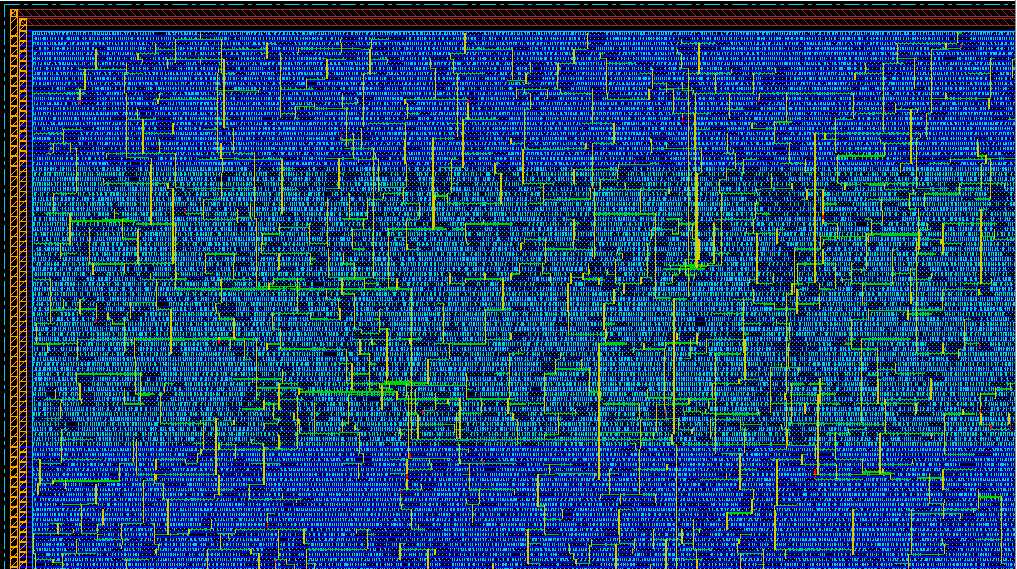
\includegraphics[width=0.85\textwidth]{CTSResult2}
}
\\
\subfigure[CTS综合后层级时钟树]{
\label{figure4.4b}
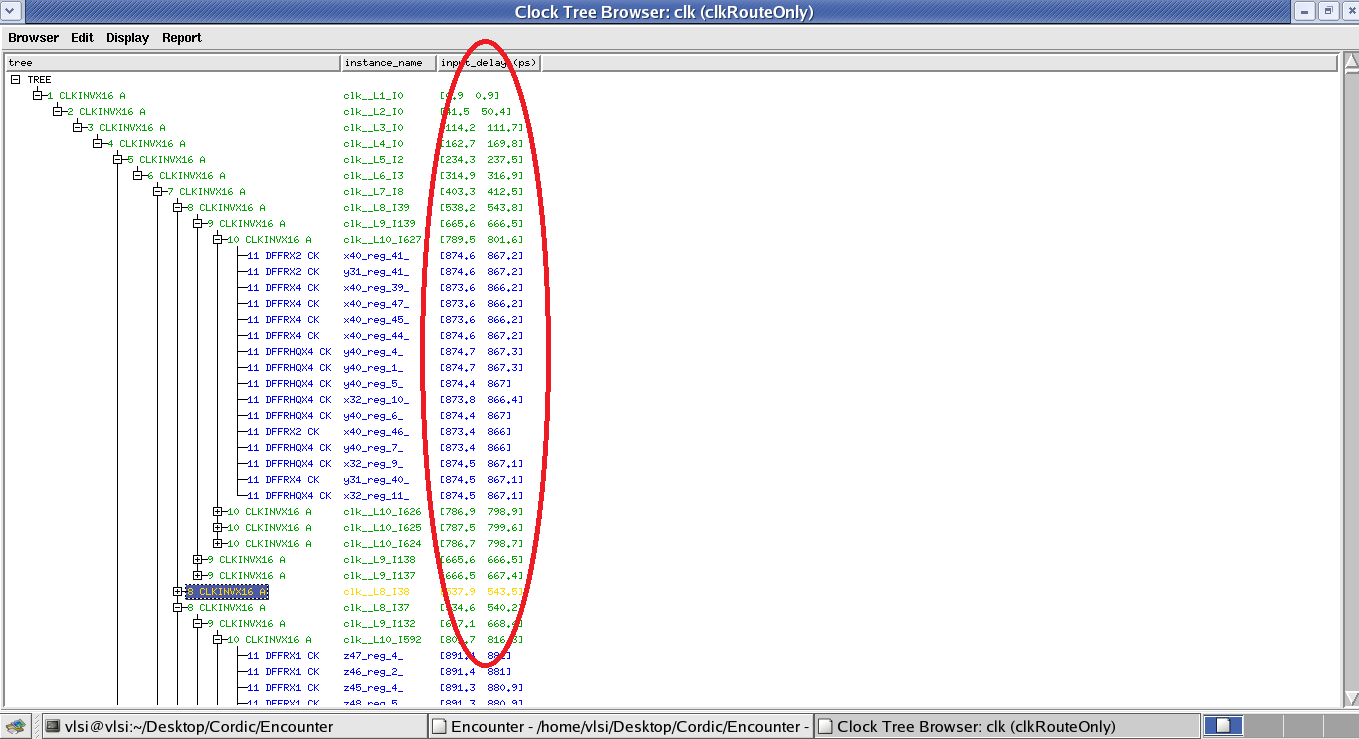
\includegraphics[width=0.85\textwidth]{clockTree1}
}

\caption{CTS综合后的结果}
\label{figure4.4}
\end{figure}

\subsection{布线}
\noindent {\bfseries 基于Encounter的布线流程如下}:
\begin{itemize}
\item 读入上一步布局以及CTS综合的结果
\item 设置布线模式
\item 布线完成后,对时序进行分析
\item 对设计进行优化\\
	\verb|optDesign -postRoute|
\item 进行SI优化\\
	\verb|optDesign -postRoute -si|
\item 做优化后的时序分析
\item 保存database
\item 在标准单元之间的空隙插入filter、金属等
\item 对走线进行DRC检查\\
	\verb|fillNotch|
\item 插入金属填充,针对较细的金属线进行密度填充
\item 对整个设计进行检查\\
	包括是否开路、悬空Pin、天线效应、最小面积、最小间距等
\item 到此Encounter的工作结束,保存database、gds网表及其它文件
\end{itemize}
\noindent {\bfseries 布线结果}:\\
\indent 这一步骤主要是在前一步CTS时钟树布线后进行,在本实验中,布线过程设置为时序驱动,且考虑天线效应。在完成布线模式设置后并布线后,对设计进行一次时序分析,此时,可以得到关于建立时间以及保持时间是否违反约束的信息等。然后对设计利用\verb|optDesign -postRoute|以及\verb|optDesign -postRoute -si|对设计进行包括拓扑效应在内的优化。最后在进行一次时序分析,保证没有时序违反,最后保存设计。接下来就是插入一些Filter以及金属填充等工作。

相应的,图\ref{figure4.5a}表示了布线结果,其中途中的前面窗口展示了布线后关于模块的一些参数信息,包括管脚的个数、资源占用率等。图\ref{figure4.5b}为金属填充后的效果图。在金属填充之前需要对设计进行微小DRC错误进行检查,这一步利用\verb|fillNotch|完成,终端的相关检查输出这里不在赘述。

布线完成后,即完成了在Encounter下的大部分工作,剩下的就是对布线结果进行相关的检测,包括是否有悬空的pin、是否存在开路、是否存在天线效应以及是否满足最小线宽、最小面积约束等。图\ref{figure4.6}表示Verify Connectivity的检查结果,从图\ref{figure4.6a}所示的界面中可以选择需要的检测选项。图\ref{figure4.7}所示为Verify Geometry的检查结果,同样的,从图\ref{figure4.7a}所示的界面中可以选择需要的检测选项等。相关检测结果表明,设计的模块没有违反上述约束的情况存在。

\begin{figure}[!hbtp]
\centering
\subfigure[初步布线结果]{
\label{figure4.5a}
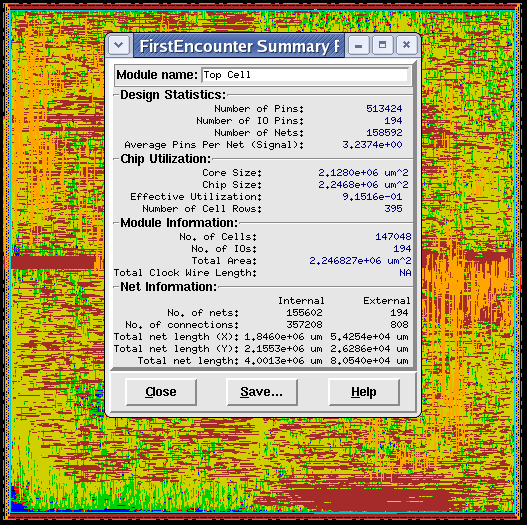
\includegraphics[width=0.4\textwidth]{route1_1}
}
\:
\subfigure[金属填充后的结果]{
\label{figure4.5b}
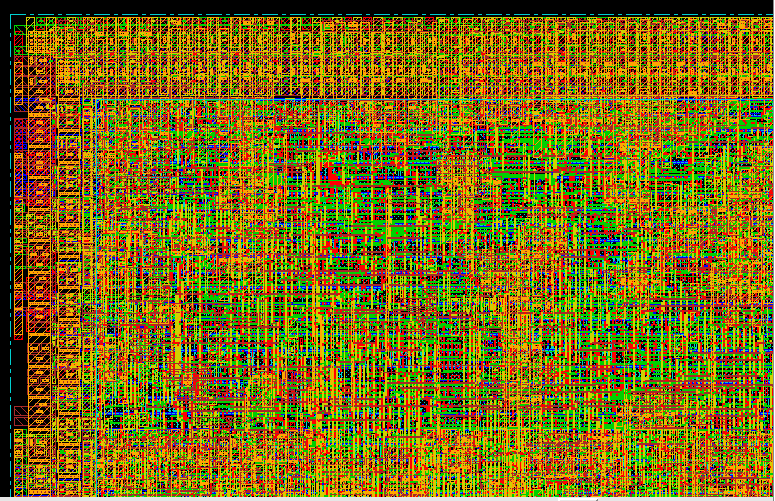
\includegraphics[width=0.4\textwidth]{metalFill2}
}
\caption{初步布线结果以及金属填充后的结果}
\label{figure4.5}
\end{figure}

\begin{figure}[!hbtp]
\centering
\subfigure[Verify Connectivity设置]{
\label{figure4.6a}
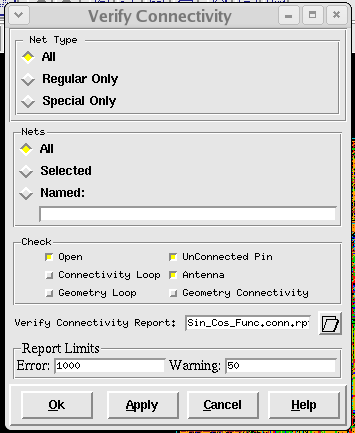
\includegraphics[width=0.4\textwidth]{verifyConnectivity1}
}
\:
\subfigure[Verify Connectivity检测结果]{
\label{figure4.6b}
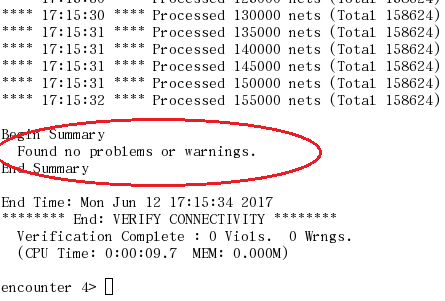
\includegraphics[width=0.4\textwidth]{verifyConnectivity2}
}
\caption{Verify Connectivity用于检测是否存在开路、悬空Pin、天线效应等}
\label{figure4.6}
\end{figure}

\begin{figure}[!hbtp]
\centering
\subfigure[Verify Connectivity设置]{
\label{figure4.7a}
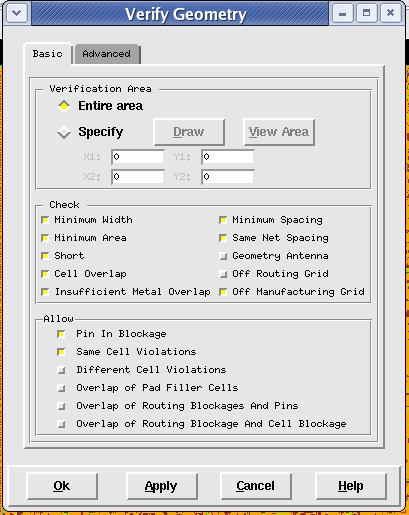
\includegraphics[width=0.4\textwidth]{verifyGeometry1}
}
\:
\subfigure[Verify Connectivity检测结果]{
\label{figure4.7b}
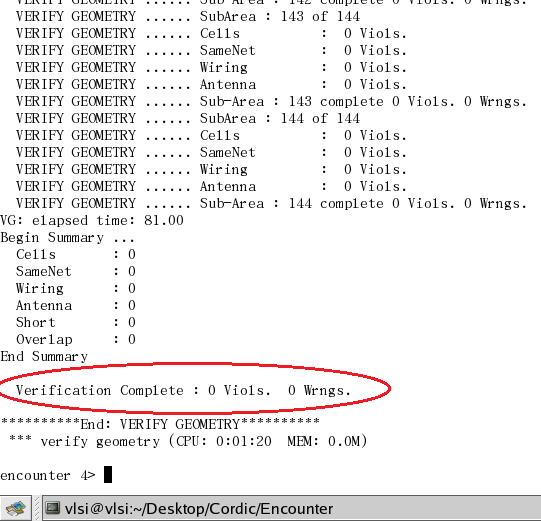
\includegraphics[width=0.4\textwidth]{verifyGeometry2}
}
\caption{Verify Geometry用于检测是否满足最小面积、线宽等约束}
\label{figure4.7}
\end{figure}

\subsection{物理验证}
\noindent {\bfseries 基于Calibre的物理验证包括DRC检查以及LVS检查等,具体流程如下}:
\begin{itemize}
\item 新建目录并启动calibre
\item 进行天线效应检查
\item 进行DRC检查
\item 进行LVS验证
\begin{itemize}
\item 对布局布线得到的.gds网表文件进行转换成.cdl网表文件\\
\verb|run_v2lvs|
\item 运行LVS进行LVS验证
\end{itemize}
\item 到此物理验证部分完成
\end{itemize}
\noindent {\bfseries 物理验证结果}:\\
\indent 物理验证主要基于Calibre工具软件完成。共检查天线效应、DRC检查、LVS验证三项检查。
图\ref{figure4.8}为天线效应的检查结果,从截图中的笑脸可以看出,设计中不存在天线效应。

在对设计进行DRC检查的时候,共出现了如图\ref{figure4.9}所示的几个错误,其中,第一个错误为\textbf{Check GT\_7 -1 result},具体错误内容为多晶硅密度错误。此外,还包括途中展开的\textbf{Check V5\_1 -48 Result}等错误。为验证出现的DRC错误是用到的库与实验设计本身存在差异造成的,也就是说是规则库的误报造成的,首先将用到的库根据具体的设计本身进行修改,然后利用Hercules工具软件对用到的库进行分析。结果表明多晶硅密度有违反的情况,而此种情况并不说明设计存在的问题,修正方法可以是对多晶硅密度进行修改,但在本次试验中,并不涉及相关内容。

最后是LVS检查,在进行LVS检查前,需要将Encounter产生的.gds网表文件转换成.cdl格式,该项工作由一个脚本完成。最后图\ref{figure4.10}显示了最后的LVS检查结果,截图表明存在Layout与源文件不一致的情况,具体表现为\textbf{mission connection},通过查看LVS输出的报告,该错误属于\textbf{Name Error(ne)},根据这一提示,通过百度、Google等查找,发现这个问题可能是由于不同工具软件之间对大小写敏感性的差异造成的。但由于对工具软件掌握不深,并没有找到如何修改这种不一致性。其次,另一篇关于Calibre工具的使用手册中给出了这种情况下,且Net中线的数值小于Source Name中的数值时的修该方法,但由于该修改过程涉及到另一工具,因此同样没有成功,因此,关于这个问题还有待进一步研究解决。

\begin{figure}[!hbtp]
\centering
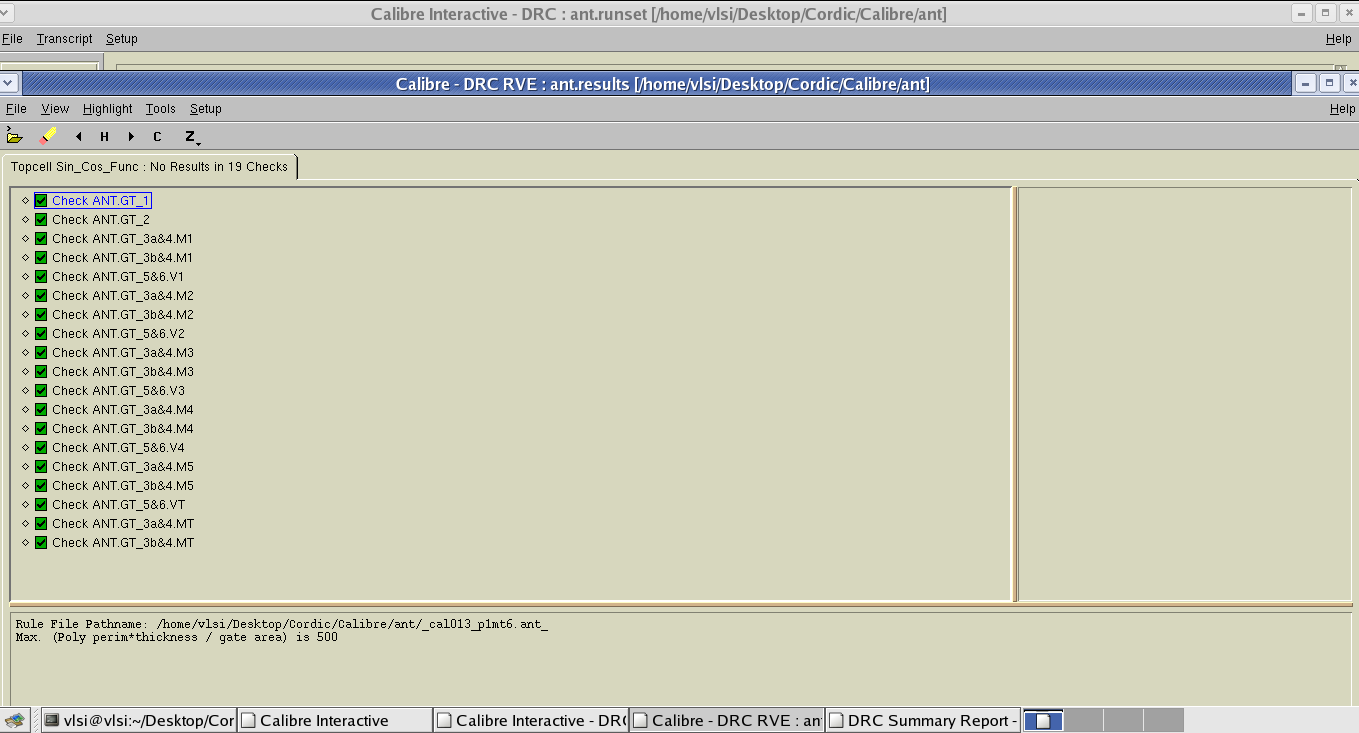
\includegraphics[width=0.9\textwidth]{ANT1}
\caption{天线效应检查结果}
\label{figure4.8}
\end{figure}


\begin{figure}[!hbtp]
\centering
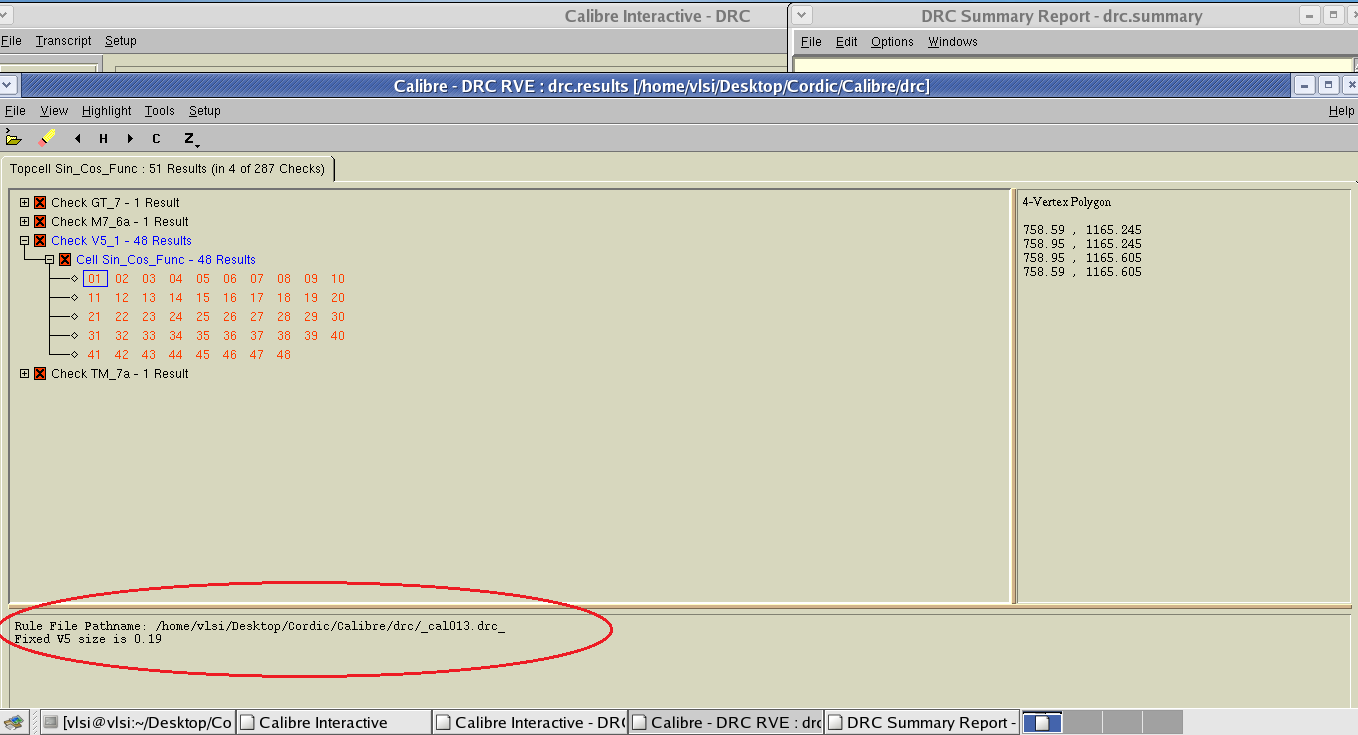
\includegraphics[width=0.9\textwidth]{DRC1}
\caption{DRC检查结果}
\label{figure4.9}
\end{figure}


\begin{figure}[!hbtp]
\centering
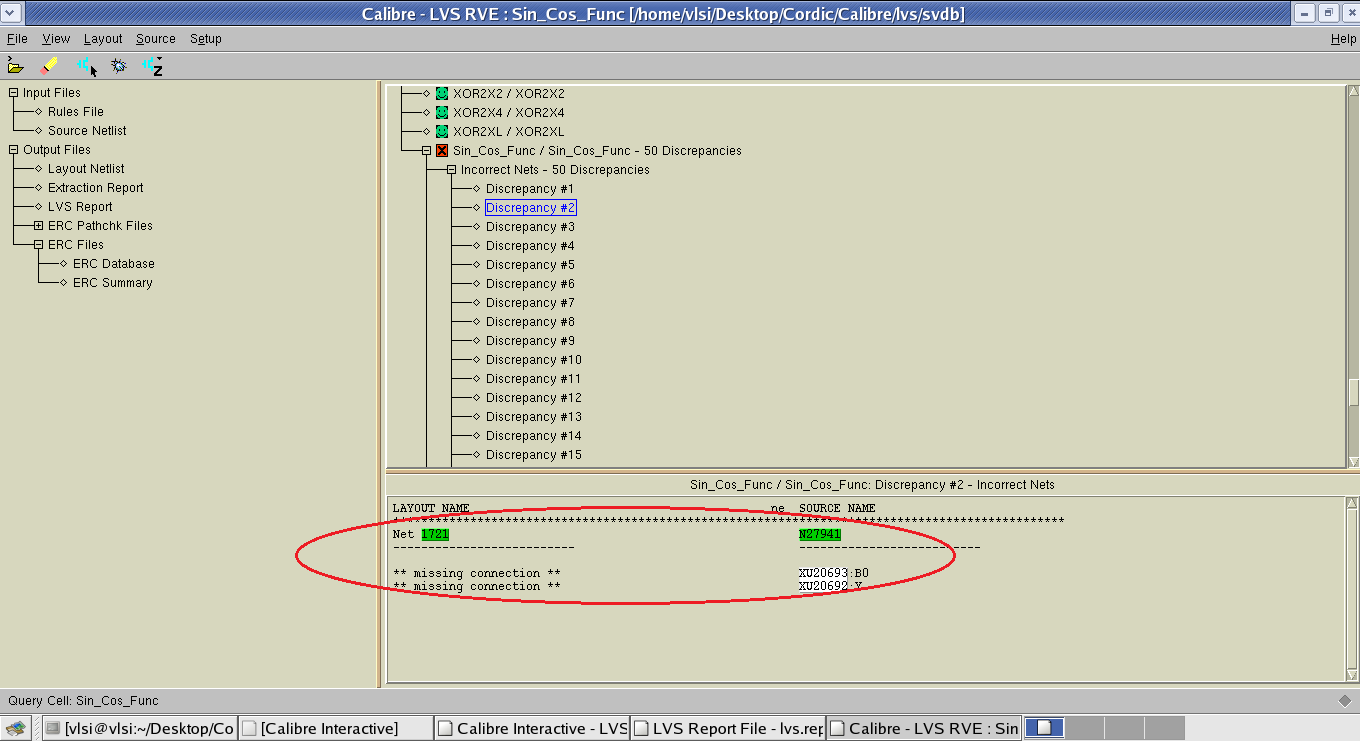
\includegraphics[width=0.9\textwidth]{LVS1}
\caption{LVS检查结果}
\label{figure4.10}
\end{figure}

\section{总结}
本章节主要是基于Cordic模块的前端设计流程进行的后端物理设计,包括四个主要的步骤:布局规划(Floorplan), 布局与CTS时钟树综合,布线,物理验证等。主要用到的工具软件包括Encounter以及Calibre。


\chapter{总结}
通过完成本次实验,熟悉了数字集成电路的完整设计流程,包括最开始的基于Verilog的模块功能的实现,然后是借助NC工具软件对设计进行模拟验证,以保证设计功能的正确性,具体的,在本实验中,应保证Cordic模块在$0 \sim \pi/2$范围内的输入角度,能正确计算其sin, cos值。
同时,为保证功能正确性,应该尽可能多的对设计进行测试,即保证足够的验证覆盖率,在本实验中,主要采用临界值与普通值相互结合的验证,临界值包括输入0度时的输出等,此外,还包括输入为$30^{\circ}, 45^{\circ}, 60^{\circ}$, 结果表明,设计的模块对于非临界值情况下具有较好的计算效果,但对于临界值输入情况下,sin值计算误差较大,关于这一点还需要进一步改进。
在保证设计功能正确的基础上,基于DC工具软件完成了对设计的逻辑综合,其过程为将HDL代码转化为网表输出。该过程中,需要用到工艺库、链接库等,完成从HDL到网表的映射。同时,该过程中需要设置模块的综合用到的时钟周期,时钟周期的大小会得到不同方向的综合结果,其过程主要是平衡时序-面积之间的矛盾。最后,综合的结果为生成一个.sv格式的网标文件,该文件作为后续物理设计的输入数据需要用到。

在完成前端设计流程的基础上,本实验又进行了该模块的后端物理设计,包括第四章节中介绍的几个主要步骤。这里就不在赘述了。

总的来说,本次实验还可以在一下几个方面进行改进:
\begin{itemize}
\item 设计的模块在临界值输入情况下,计算结果有待进一步改进;同时,下一步的工作可以是基于C/C++编写黄金模型进行验证。
\item 在布局布线后,出现时序违反的情况,虽然在实验过程中,通过增大时钟周期减轻了违反的程度,但还没有一个根本有效的措施,后续工作可以是重新对模块进行设计,以新的实现结构来消除时序违反。
\item 在物理验证阶段,出现LVS检查不一致的错误,关于这个错误,虽然在网上找到了一些相关的解决措施,但由于时间有限且对工具理解不够深刻导致还没有解决相关错误,这也将是下一步可以改进的地方。
\end{itemize}

\nocite{*}
\bibliography{references}

\appendix
\section*{附录: 基于C++的Cordic实现}\label{AppendixA}
\addcontentsline{toc}{chapter}{附录 A}
\lstdefinestyle{customCpp}{
 belowcaptionskip=1\baselineskip,
  breaklines=true,
  frame=L,
  xleftmargin=\parindent,
  language=C,
  showstringspaces=false,
  basicstyle=\footnotesize\ttfamily,
  keywordstyle=\bfseries\color{green!40!black},
  commentstyle=\itshape\color{purple!40!black},
  identifierstyle=\color{blue},
  stringstyle=\color{orange},
}
{
\lstset{style=customCpp}
\footnotesize
\begin{lstlisting}
#include <iostream>
#include <vector>

using namespace std;

// 1 bit sign bit, 1 bit integer, for example = 1
vector<long int> Atan = {0x3243F6A9, 
 0x1dac6705, 0x0fadbafd, 0x07f56ea7, 0x03feab77, 0x01ffd55c, 
 0x00fffaab, 0x007fff55, 0x003fffeb, 0x001ffffd, 0x00100000, 
 0x00080000, 0x00040000, 0x00020000, 0x00010000, 0x00008000,
 0x00004000, 0x00002000, 0x00001000, 0x00000800, 0x00000400, 
 0x00000200, 0x00000100, 0x00000080, 0x00000040, 0x00000020, 
 0x00000010, 0x00000008, 0x00000004, 0x00000002, 0x00000001,
 0x00000000
 };

int main(int argc, char **argv)
{
	long int c = 0x26DD3B6A;    // = 0.6072529350088814
	long int s = 0;

	long int c_next = c;
	long int s_next = s;

	// get the input angle 
	//long int angle = 0x3243F6A9;   // input : Pi / 4 
	long int angle = 0x2182A470;     // input : Pi / 6
	long int theta = angle;
	long int direction = 1;

	for(int i = 0; i < 32; ++i)
	{
		if(theta > 0)
			direction = 1;           // Anti-clockwise
		else
			direction = -1;          // clockwise
		c_next = c - direction * (s >> i);
		s_next = s + direction * (c >> i);

		c = c_next;
		s = s_next;

		theta -= direction * Atan[i];
	}

	cout << "cos : " << c << endl;
	cout << "sin : " << s << endl;

	return 0;
}

\end{lstlisting}
}

\end{document}